\chapter{Introducción}
\label{cap:capitulo1}
\setcounter{page}{1}

\begin{flushright}
\begin{minipage}[]{10cm}
\emph{El éxito es la capacidad de ir de fracaso en fracaso sin perder el entusiasmo.}\\
\end{minipage}\\

Winston Churchill\\
\end{flushright}


\section{Robótica}
\label{sec:rob}
La robótica es la ciencia encargada del diseño, construcción y programación de robots. Se entiende por robot, a una máquina programable 
capaz de llevar a cabo tareas de forma autónoma o asistida capaz de percibir su entorno mediante sensores e interactuar con él mediante 
actuadores.\\
Pese a la creencia popular, esta disciplina se remonta a la antigüedad, donde se encuentran referencias a autómatas y dispositivos mecánicos diseñados 
que tratan de imitar acciones humanas. Sin embargo, no es hasta mediados del siglo XX cuando surge el concepto de robot tal y como los conocemos hoy en día. 
En 1954, George Devol y Joseph Engelberger desarrollaron el primer robot industrial programable llamado Unimate \ref{fig:unimate}, el cual fue usado en una fábrica General Motors 
para realizar tareas de soldadura en la línea de producción de automóviles. Este hito, marcó el comienzo de la automatización industrial y sentó las bases para 
el desarrollo futuro de robots industriales.
\begin{figure} [ht!]
  \begin{center}
    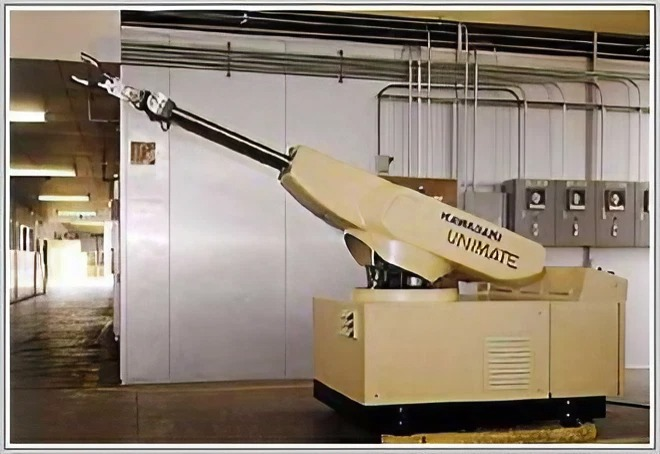
\includegraphics[width=7cm]{figs/unimate.jpg}
  \end{center}
  \caption{Robot Unimate}
  \label{fig:unimate}
\end{figure}\ 
\\
En las décadas posteriores, se produjeron numerosos avances en robótica. Se desarrollaron robots cada vez más sofisticados, que cubrian una amplia gama de tareas más allá de la 
automatización industrial. Un claro ejemplo de ello, fue el robot Shakey \ref{fig:shakey}, desarrollado por el laboratorio de investigación de la universidad de Stanford en 1966. Se trataba 
de un robot cuyo único propósito era navegar autónomamente en una sala con obstáculos gracias al uso de sensores y el uso de algoritmos de planificación.
\begin{figure} [ht!]
  \begin{center}
    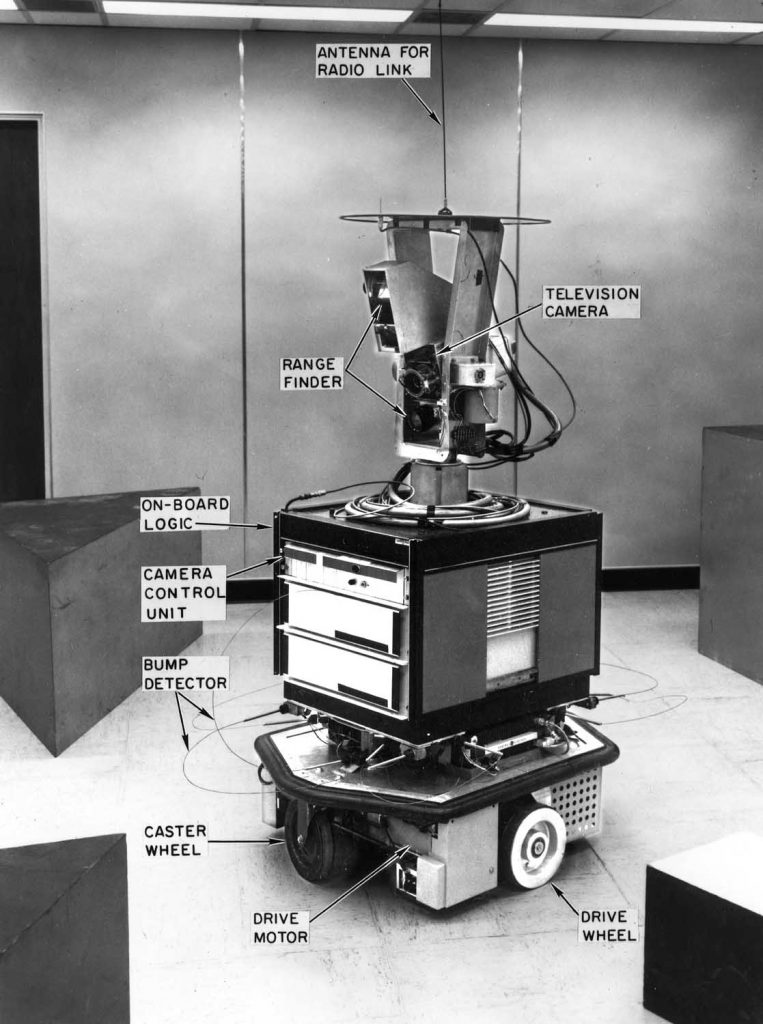
\includegraphics[width=7cm]{figs/shakey.jpg}
  \end{center}
  \caption{Robot Shakey}
  \label{fig:shakey}
\end{figure}\
\\ 
En la década de 1970, el uso de robot industriales se había disparado en todo el mundo. Estos robots, conocidos como robots manipuladores, fueron utilizados para 
realizar todo tipo de tareas repetitivas y peligrosas en fábricas.
\\
En las últimas décadas, la robótica ha seguido avanzando a pasos agigantados. Los avances en la capacidad de cómputo, el aprendizaje automático y la visión 
artificial han permitido el desarrollo de robots cada vez más inteligentes.
\\
En la actualidad, la robótica se está presente en numerosos sectores, abarcando una gran variedad de aplicaciones. Estaa versatilidad ha llevado al surgimiento 
de diversos grupos y categorías que nos permiten clasificar las diferentes tipos de robots. 
\newpage

\subsection{Robótica de servicio}
Un robot de servicio es un tipo de robot diseñado para realizar tareas en beneficio de los seres humanos. Estos robots están 
destinados a interactuar directamente con las personas por lo que están equipados con gran variedad de sensores, actuadores y sistemas de 
inteligencia artificial que les permiten percibir y comprender el entorno que los rodea. 
En función de su ámbito de uso, pueden llegar a realizar una amplia gama de tareas, como limpieza y mantenimiento del hogar, 
asistencia en la intervención médica, entrega de alimentos y productos, cuidado de personas mayores, entre otros.

\subsubsection{Robots de campo}
Se considera robot de campo a un robot diseñado para su uso en exterior, bajo unas duras condiciones. Se trata de un sector hetereogeneo en el cual se engloban los 
robots espaciales, agrícolas, búsqueda y rescate, inspección de instalaciones, minería, submarinos y conducción autónoma.
\begin{figure} [ht!]
  \centering    
  \subfigure[NASA Opportunity]{\label{fig:opportunity}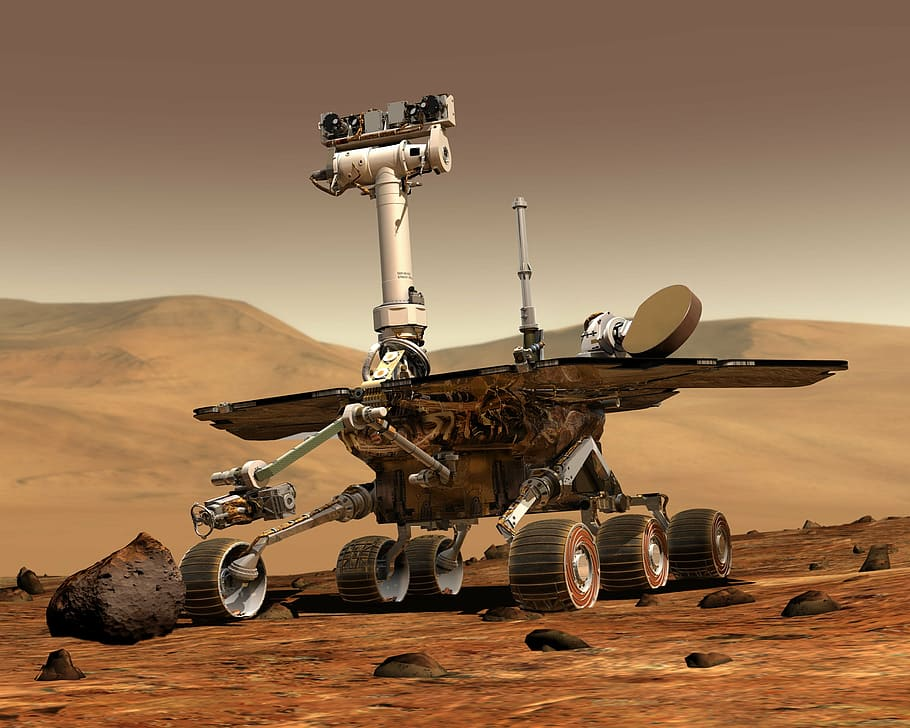
\includegraphics[width=0.25\linewidth ]{figs/rover.jpg}}
  \hspace{3cm}
  \subfigure[Tractor autónomo]{\label{fig:roomba_agua}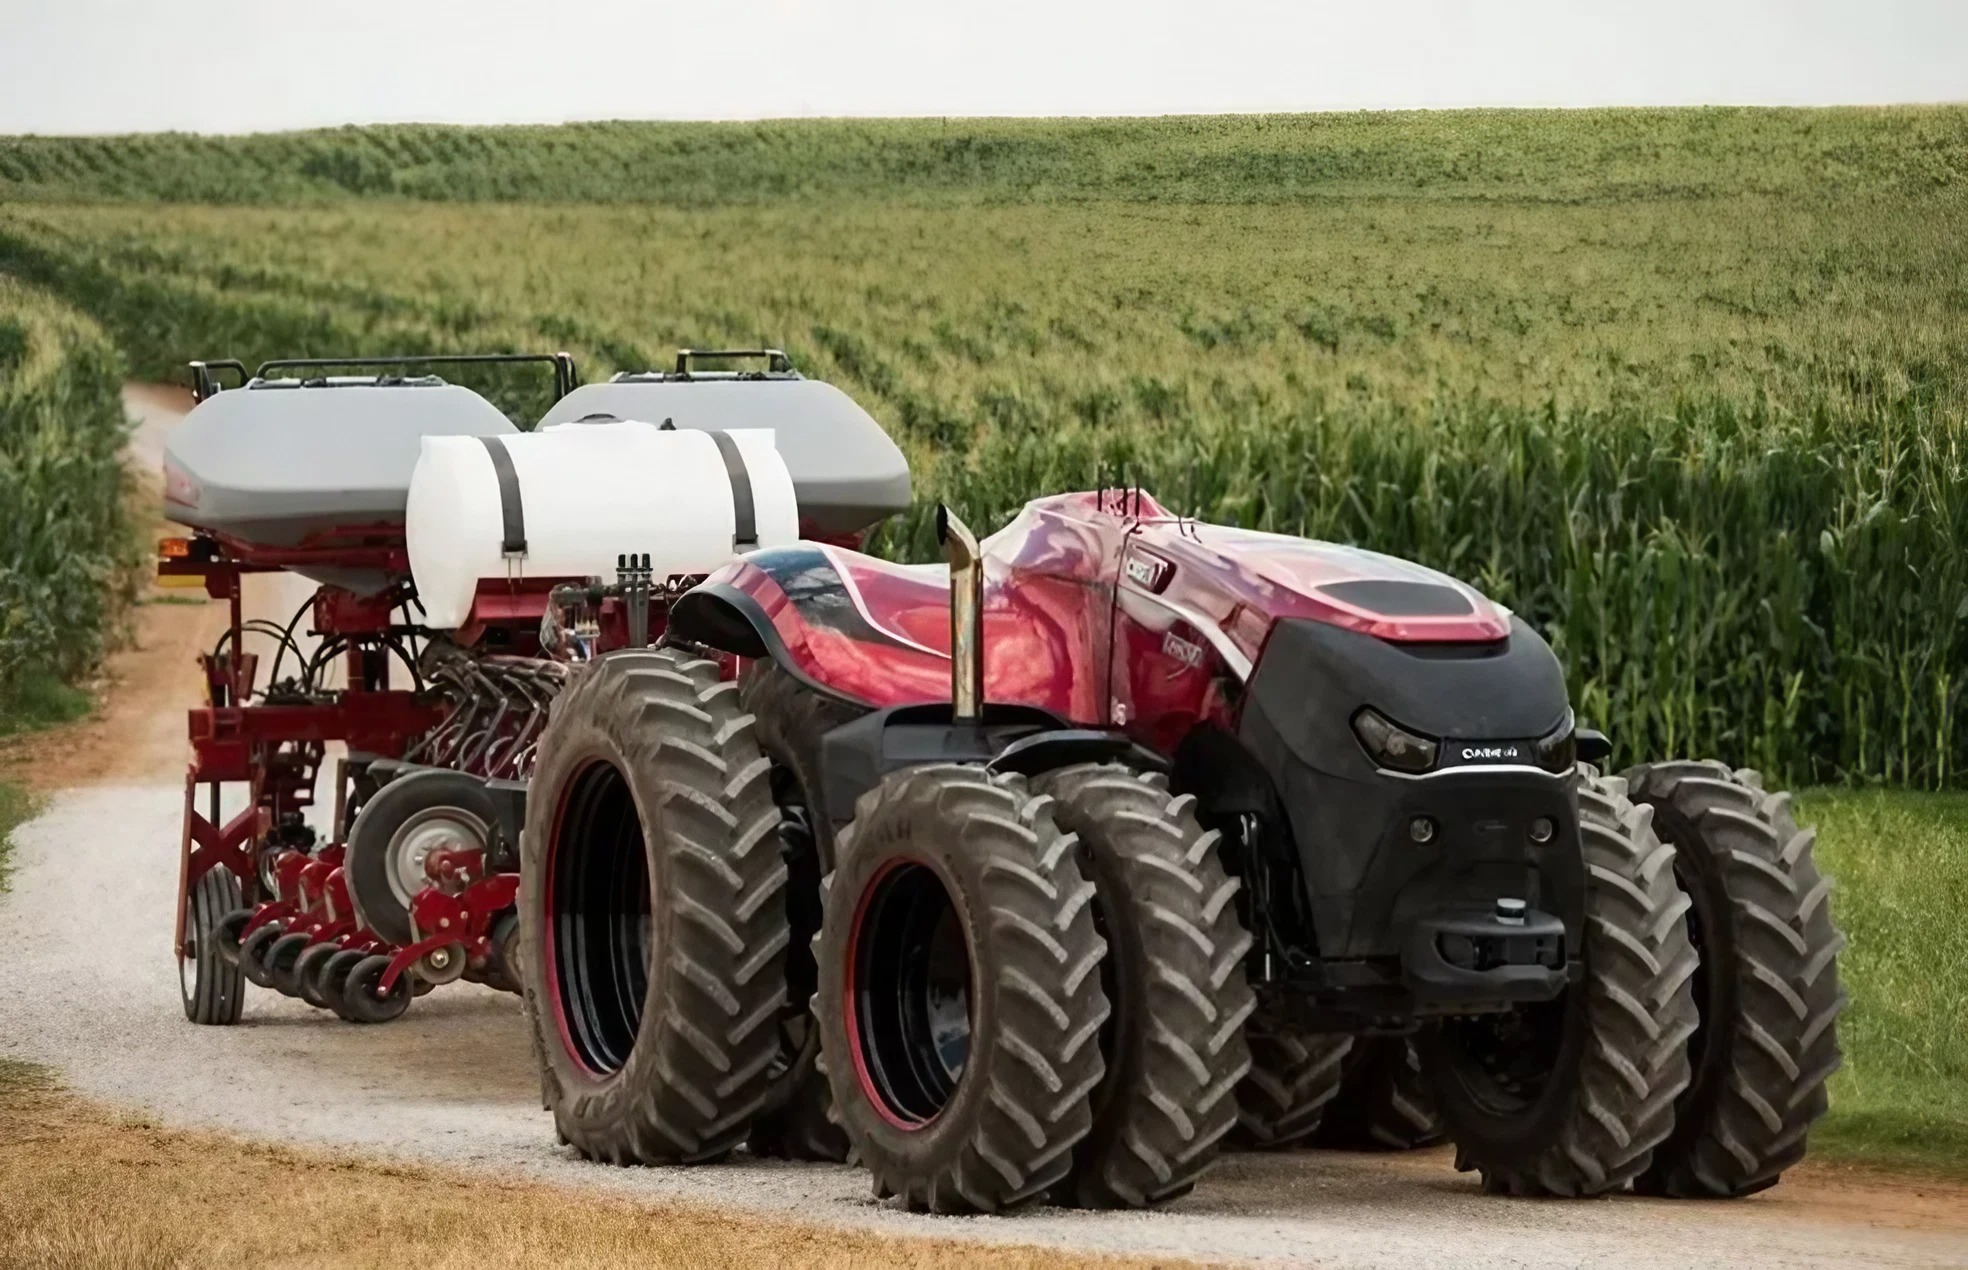
\includegraphics[width=0.25\linewidth]{figs/tractor.jpg}}
  \hspace{3cm}
  \subfigure[Drone de rescate]{\label{fig:drone}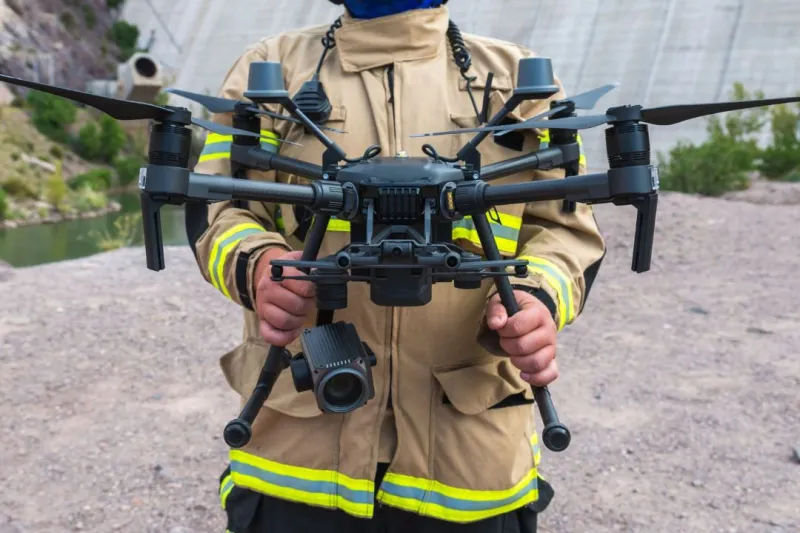
\includegraphics[width=0.25\linewidth]{figs/drone.jpg}}
  \hspace{3cm}
  \subfigure[ROV Victor 6000]{\label{fig:rov}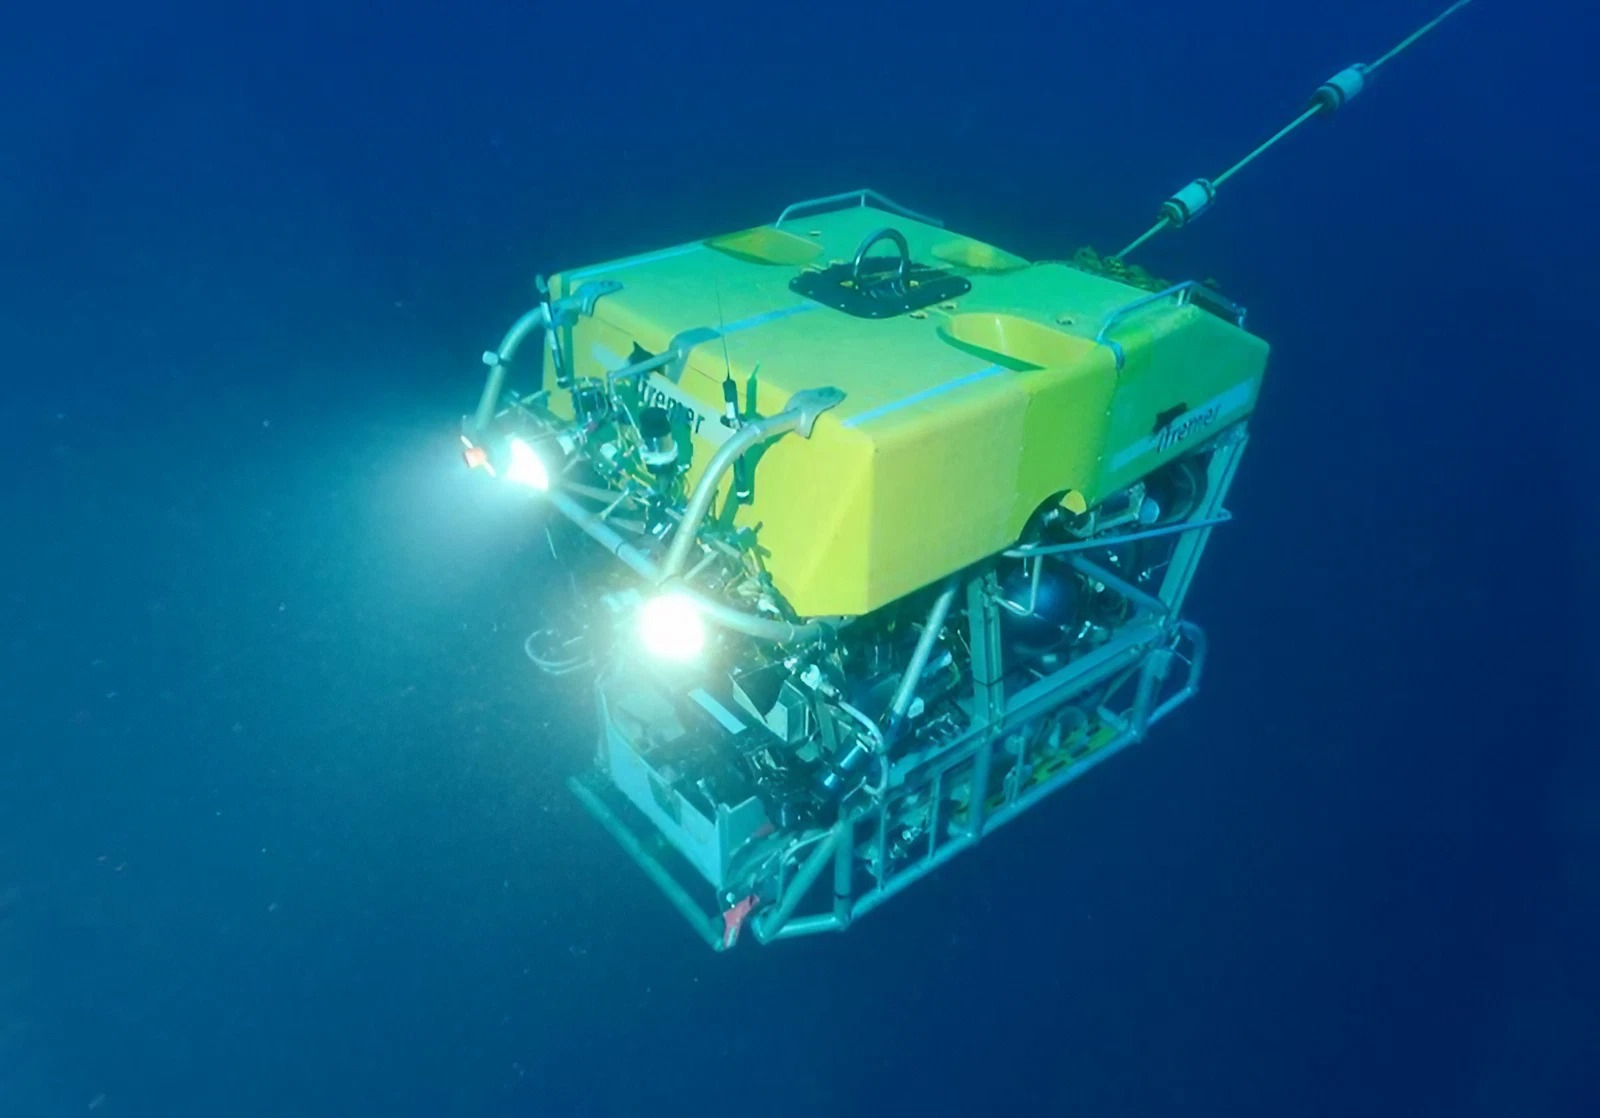
\includegraphics[width=0.25\linewidth]{figs/rov.jpg}}
  \hspace{3cm}
  \subfigure[Boston Dynamics Spot]{\label{fig:spot}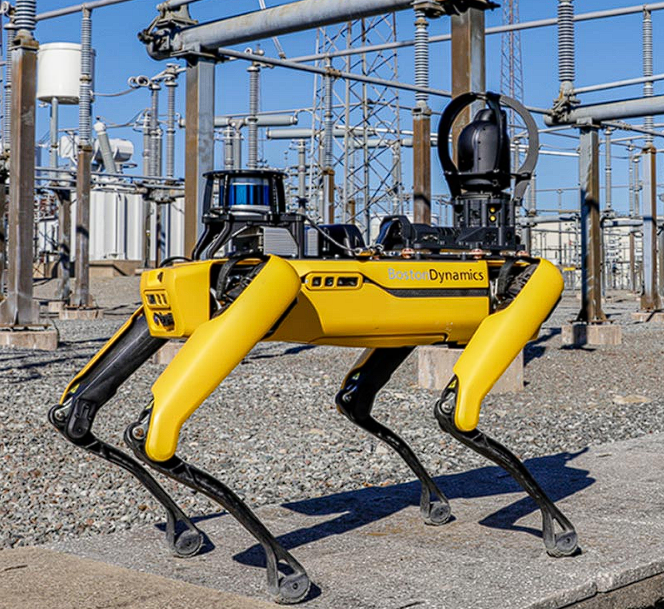
\includegraphics[width=0.25\linewidth]{figs/spot.png}}
  \hspace{3cm}
  \subfigure[Waymo]{\label{fig:autopilot}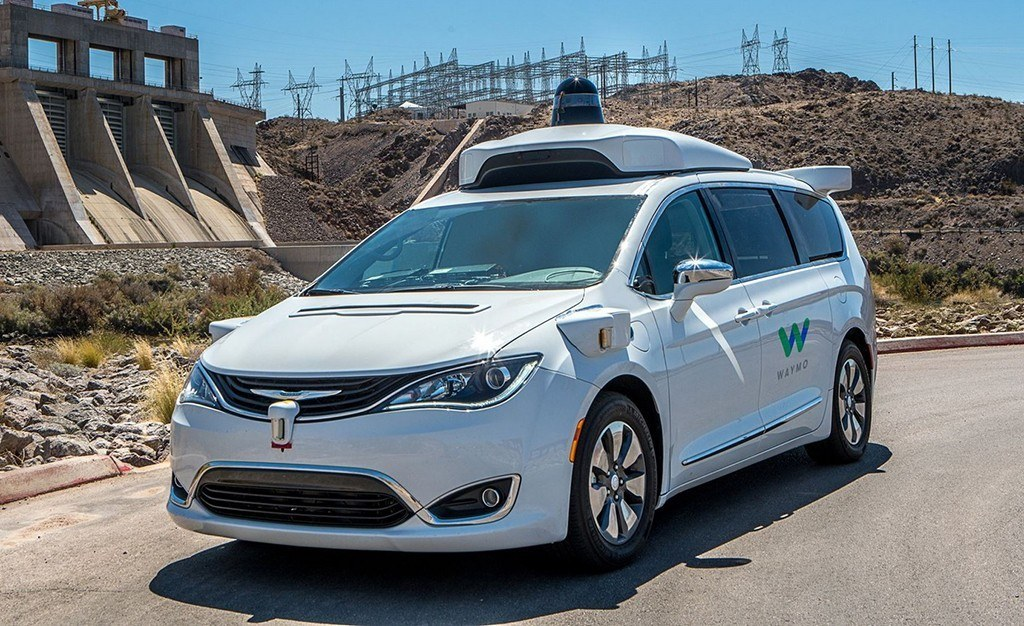
\includegraphics[width=0.25\linewidth]{figs/waymo.jpg}}
  \caption{Robots de campo}
\end{figure}

\subsubsection{Robots de limpieza}
Son aquellos robots creados para eliminar la suciedad en hogares y empresas. En función de sus características, pueden ser usados para aspirar y fregar el suelo, o incluso,
para limpiar los cristales exteriores de los edificios. Se trata de una tecnología asentada y robusta que a día de hoy cuenta con más de 20 años en el mercado. Pese a esto, 
se pueden encontrar diferentes categorías de robot en función de las necesidades. En la actualidad, integran cada vez más sensores para realizar una limpieza más eficaz y 
en entornos más imprevisibles (cables, animales, objetos tirados, etc).

\begin{figure} [ht!]
  \centering    
  \subfigure[Roomba J7+]{\label{fig:roomba}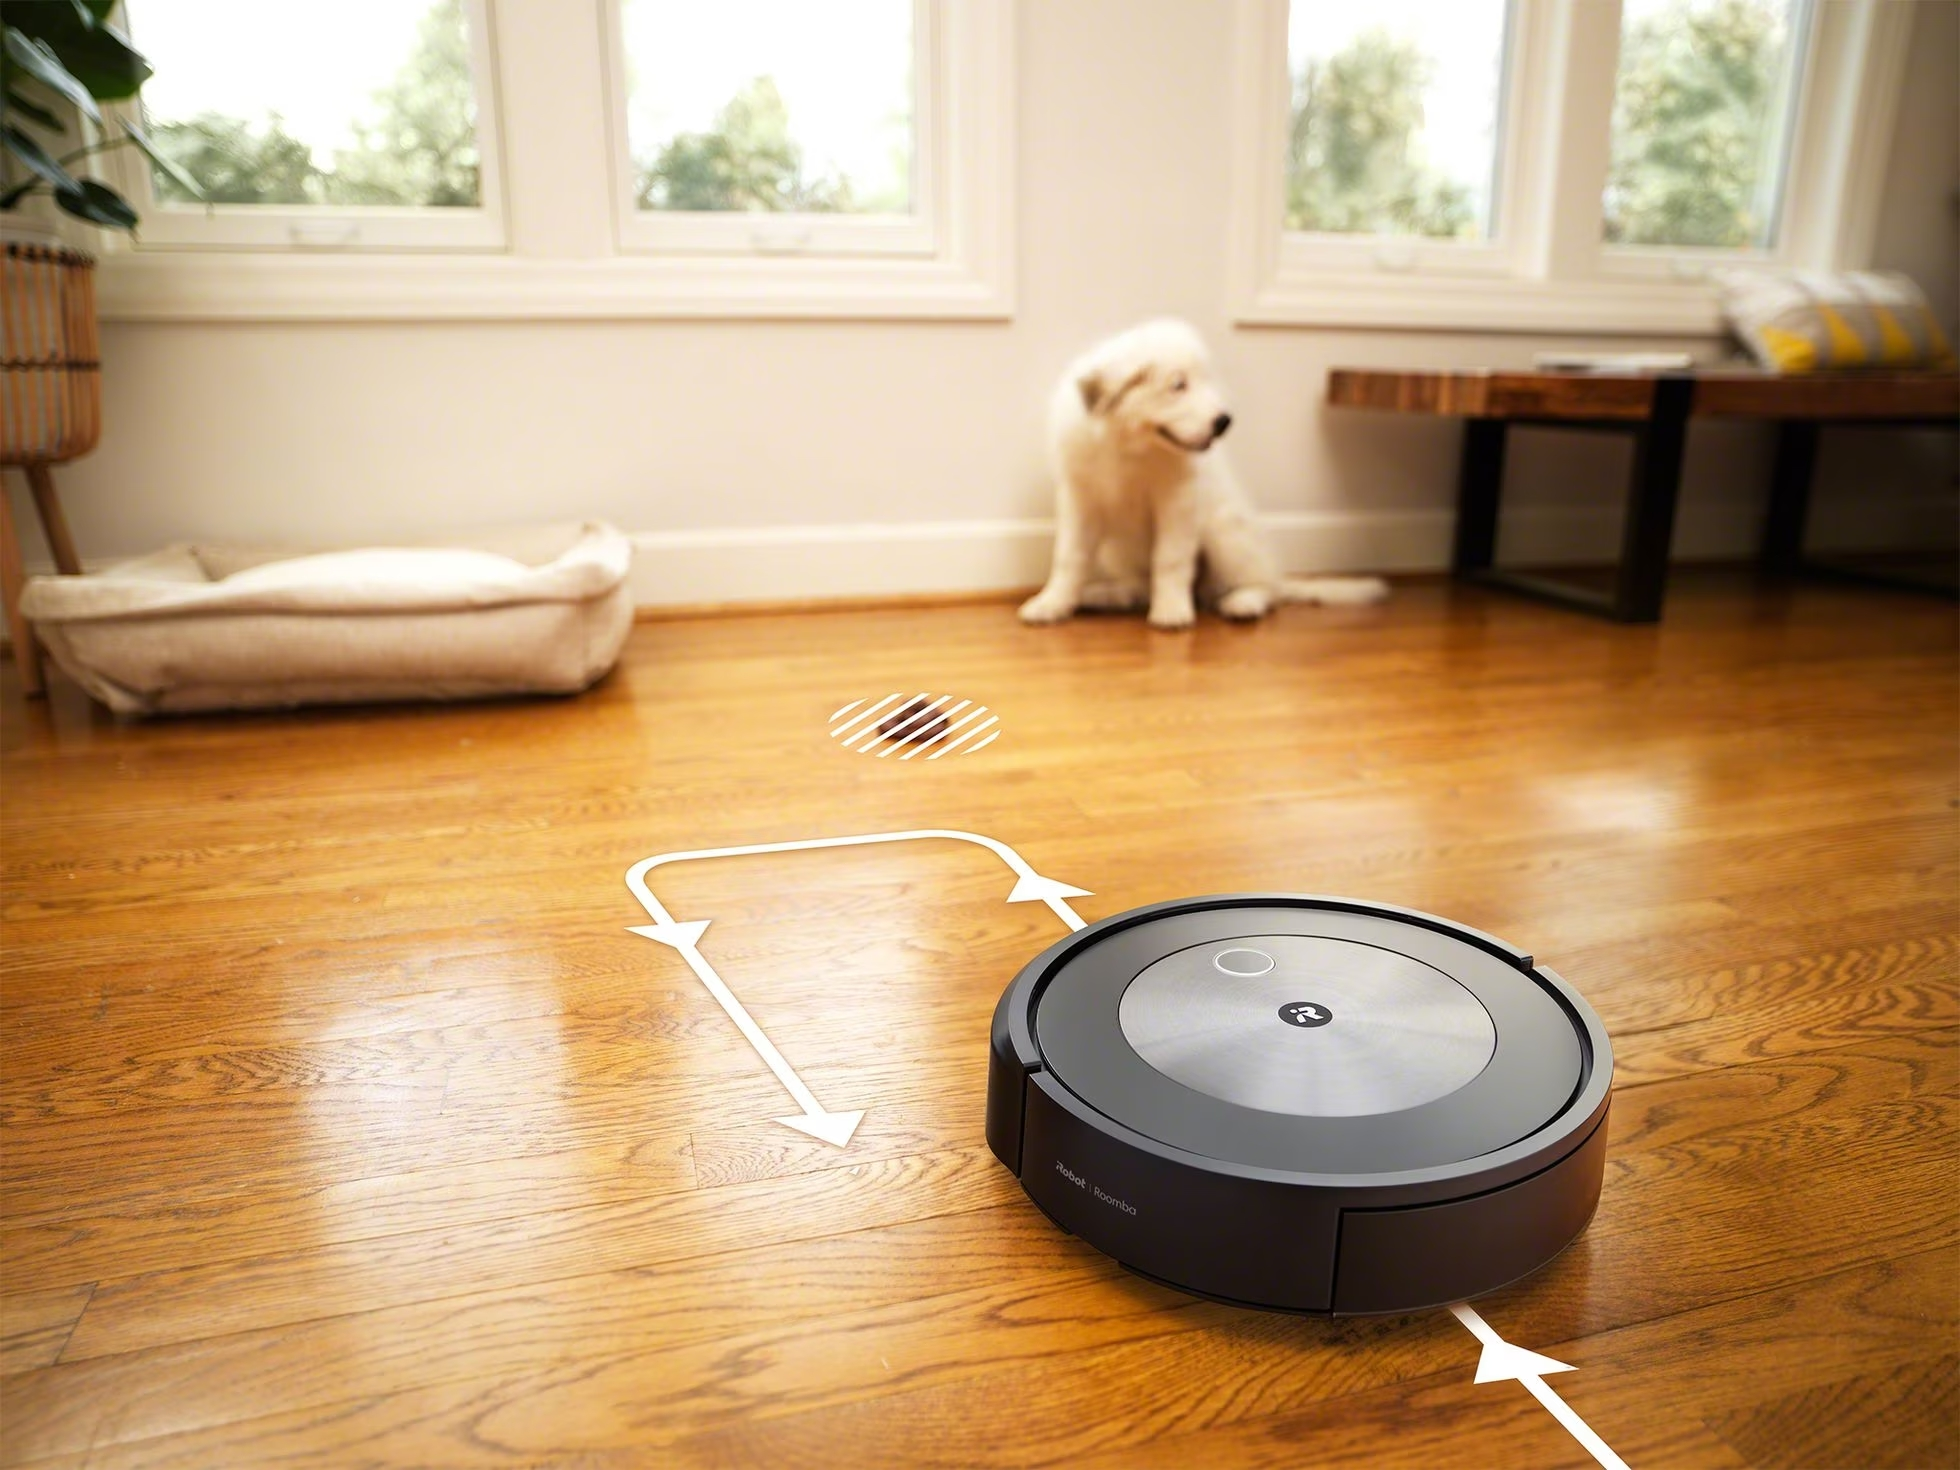
\includegraphics[width=0.25\linewidth ]{figs/roomba.jpg}}
  \hspace{1cm}
  \subfigure[Roomba Braava]{\label{fig:roomba_agua}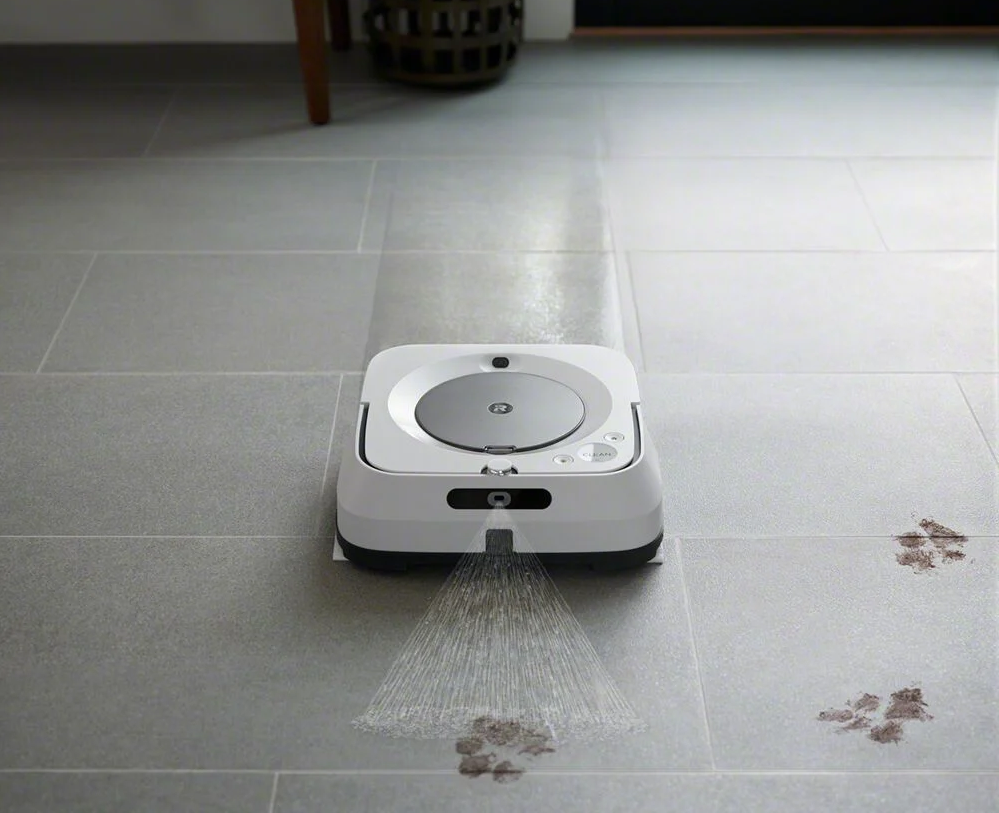
\includegraphics[width=0.25\linewidth]{figs/roombaAgua.jpg}}
  \hspace{1cm}
  \subfigure[Hobot 388]{\label{fig:hobot}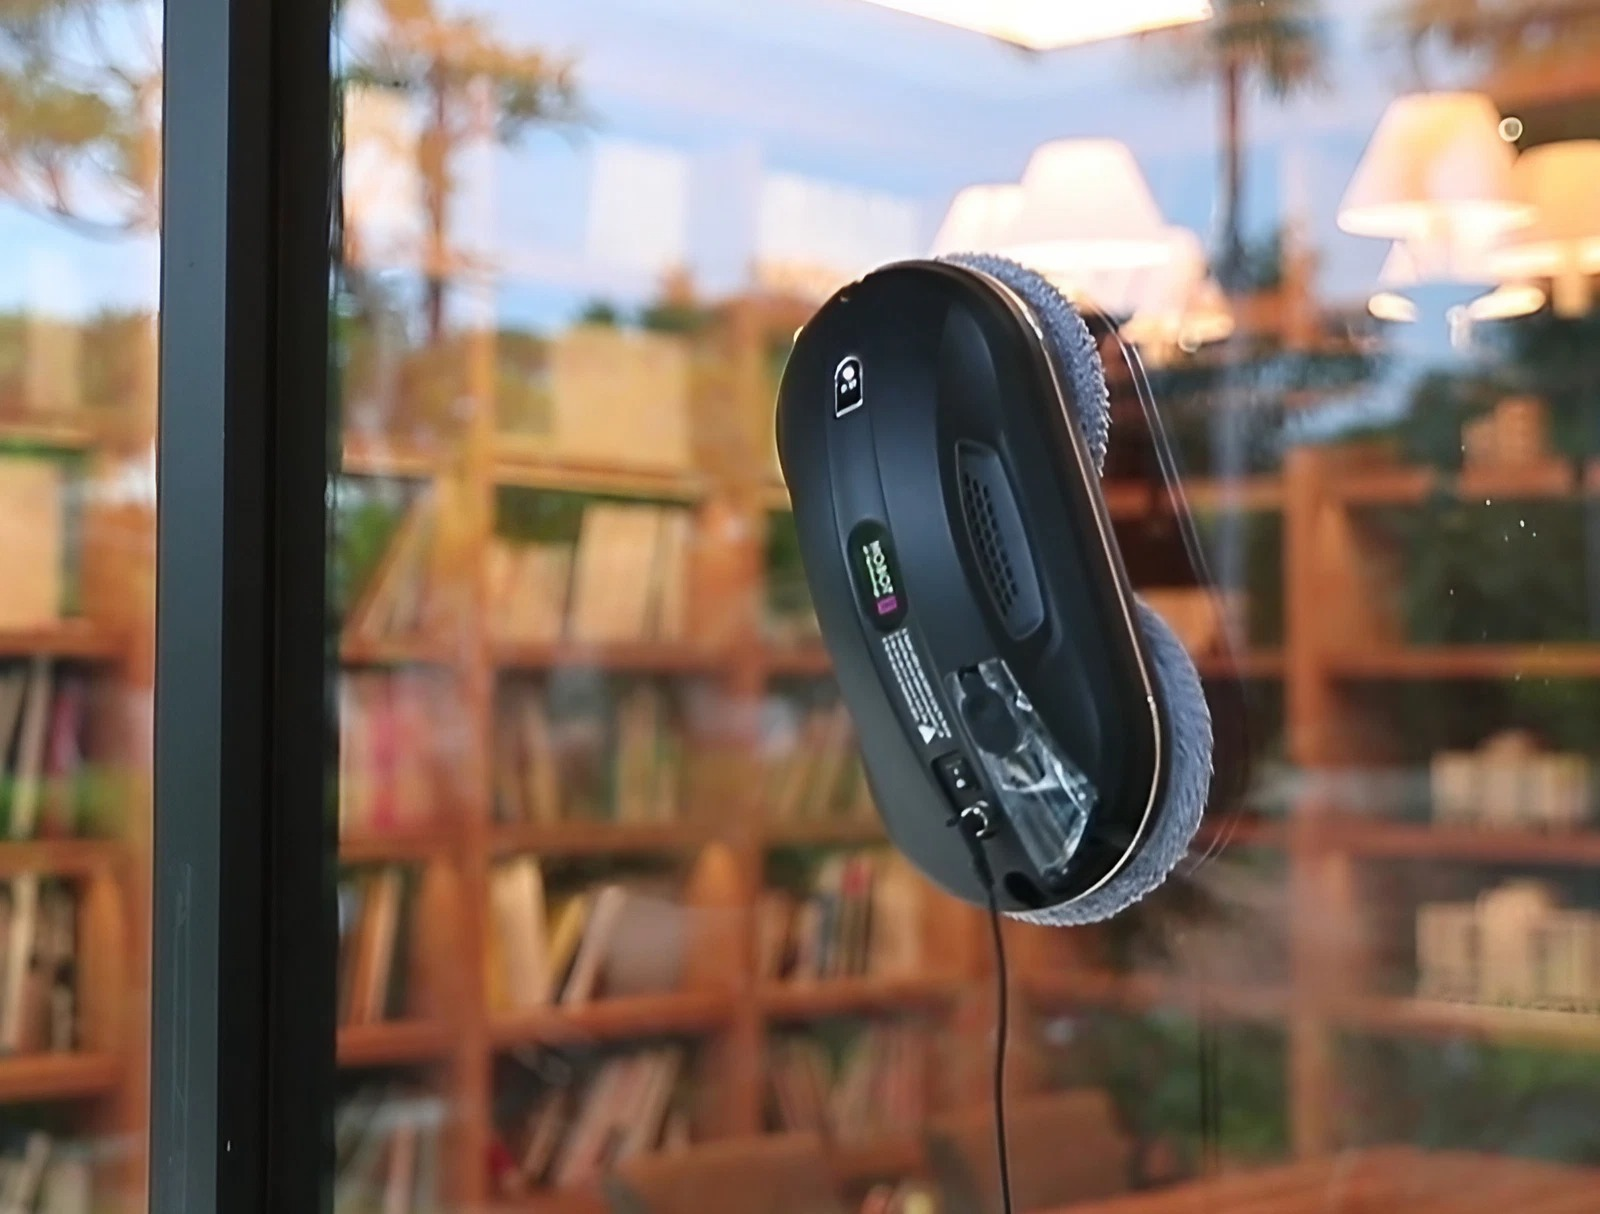
\includegraphics[width=0.25\linewidth]{figs/hobot.jpg}}
  \caption{Robots de limpieza}
\end{figure}

\subsubsection{Robots de entretenimiento}
Los robots de entretenimiento son máquinas diseñadas para proporcionar diversión y compañía a las personas. Estos robots están equipados con capacidades y 
características específicas que los hacen adecuados para interactuar con las personas. Tienen una apariencia amigable y agradable. Están pensados para 
evitar el efecto del Valle Inquietante. Esta teoría sugiere que a medida que los robots se vuelven mas humanos en apariencia y comportamiento, la respuesta 
emocional de las personas hacia ellos es más negativa, antes de volver a ser positiva a medida que se vuelven prácticamente 
indistinguibles de los seres humanos reales.
\begin{figure} [ht!]
  \centering    
  \subfigure[Aibo Sony]{\label{fig:aibo}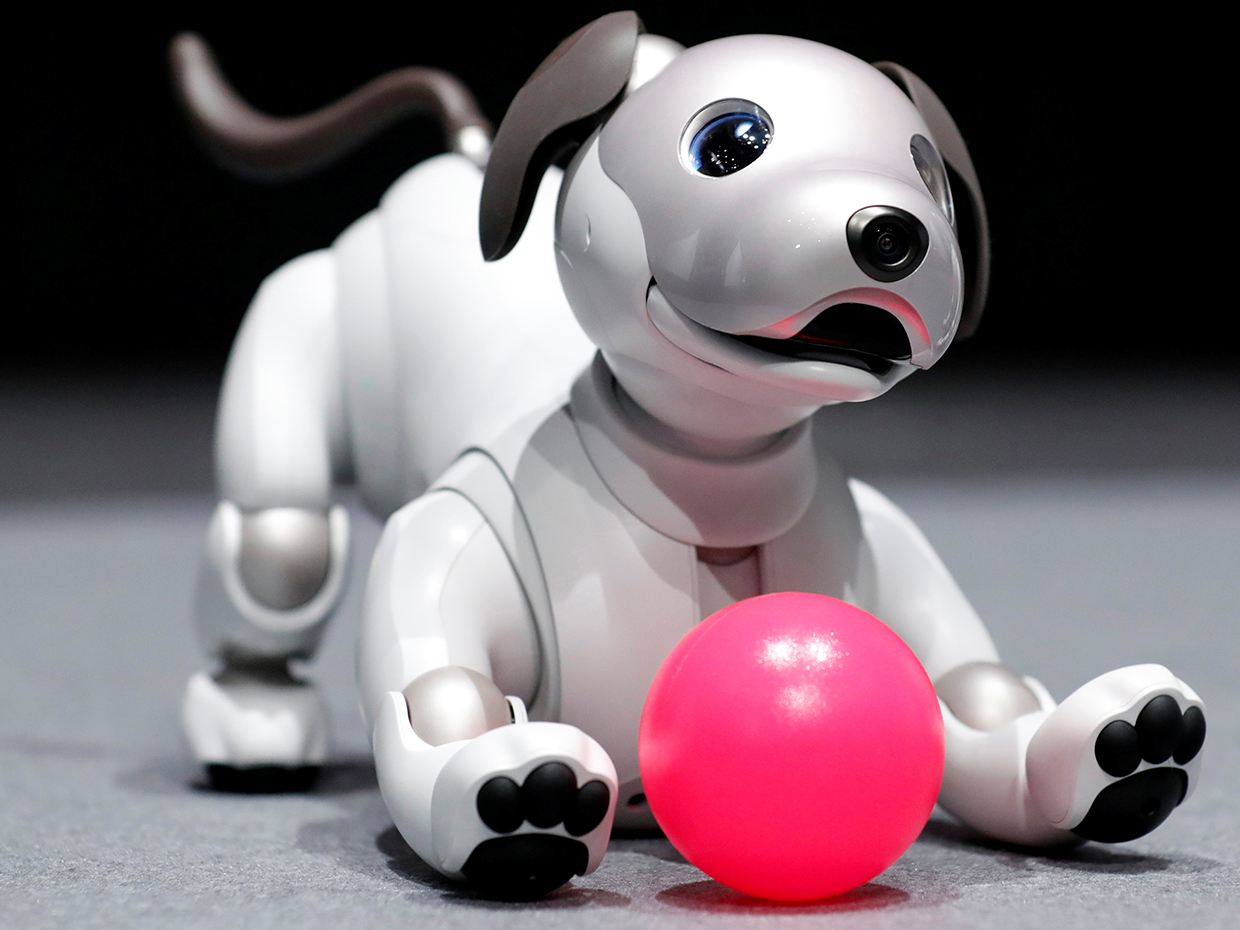
\includegraphics[width=0.28\linewidth ]{figs/aibo.jpeg}}
  \hspace{1cm}
  \subfigure[Foca Paro]{\label{fig:paro}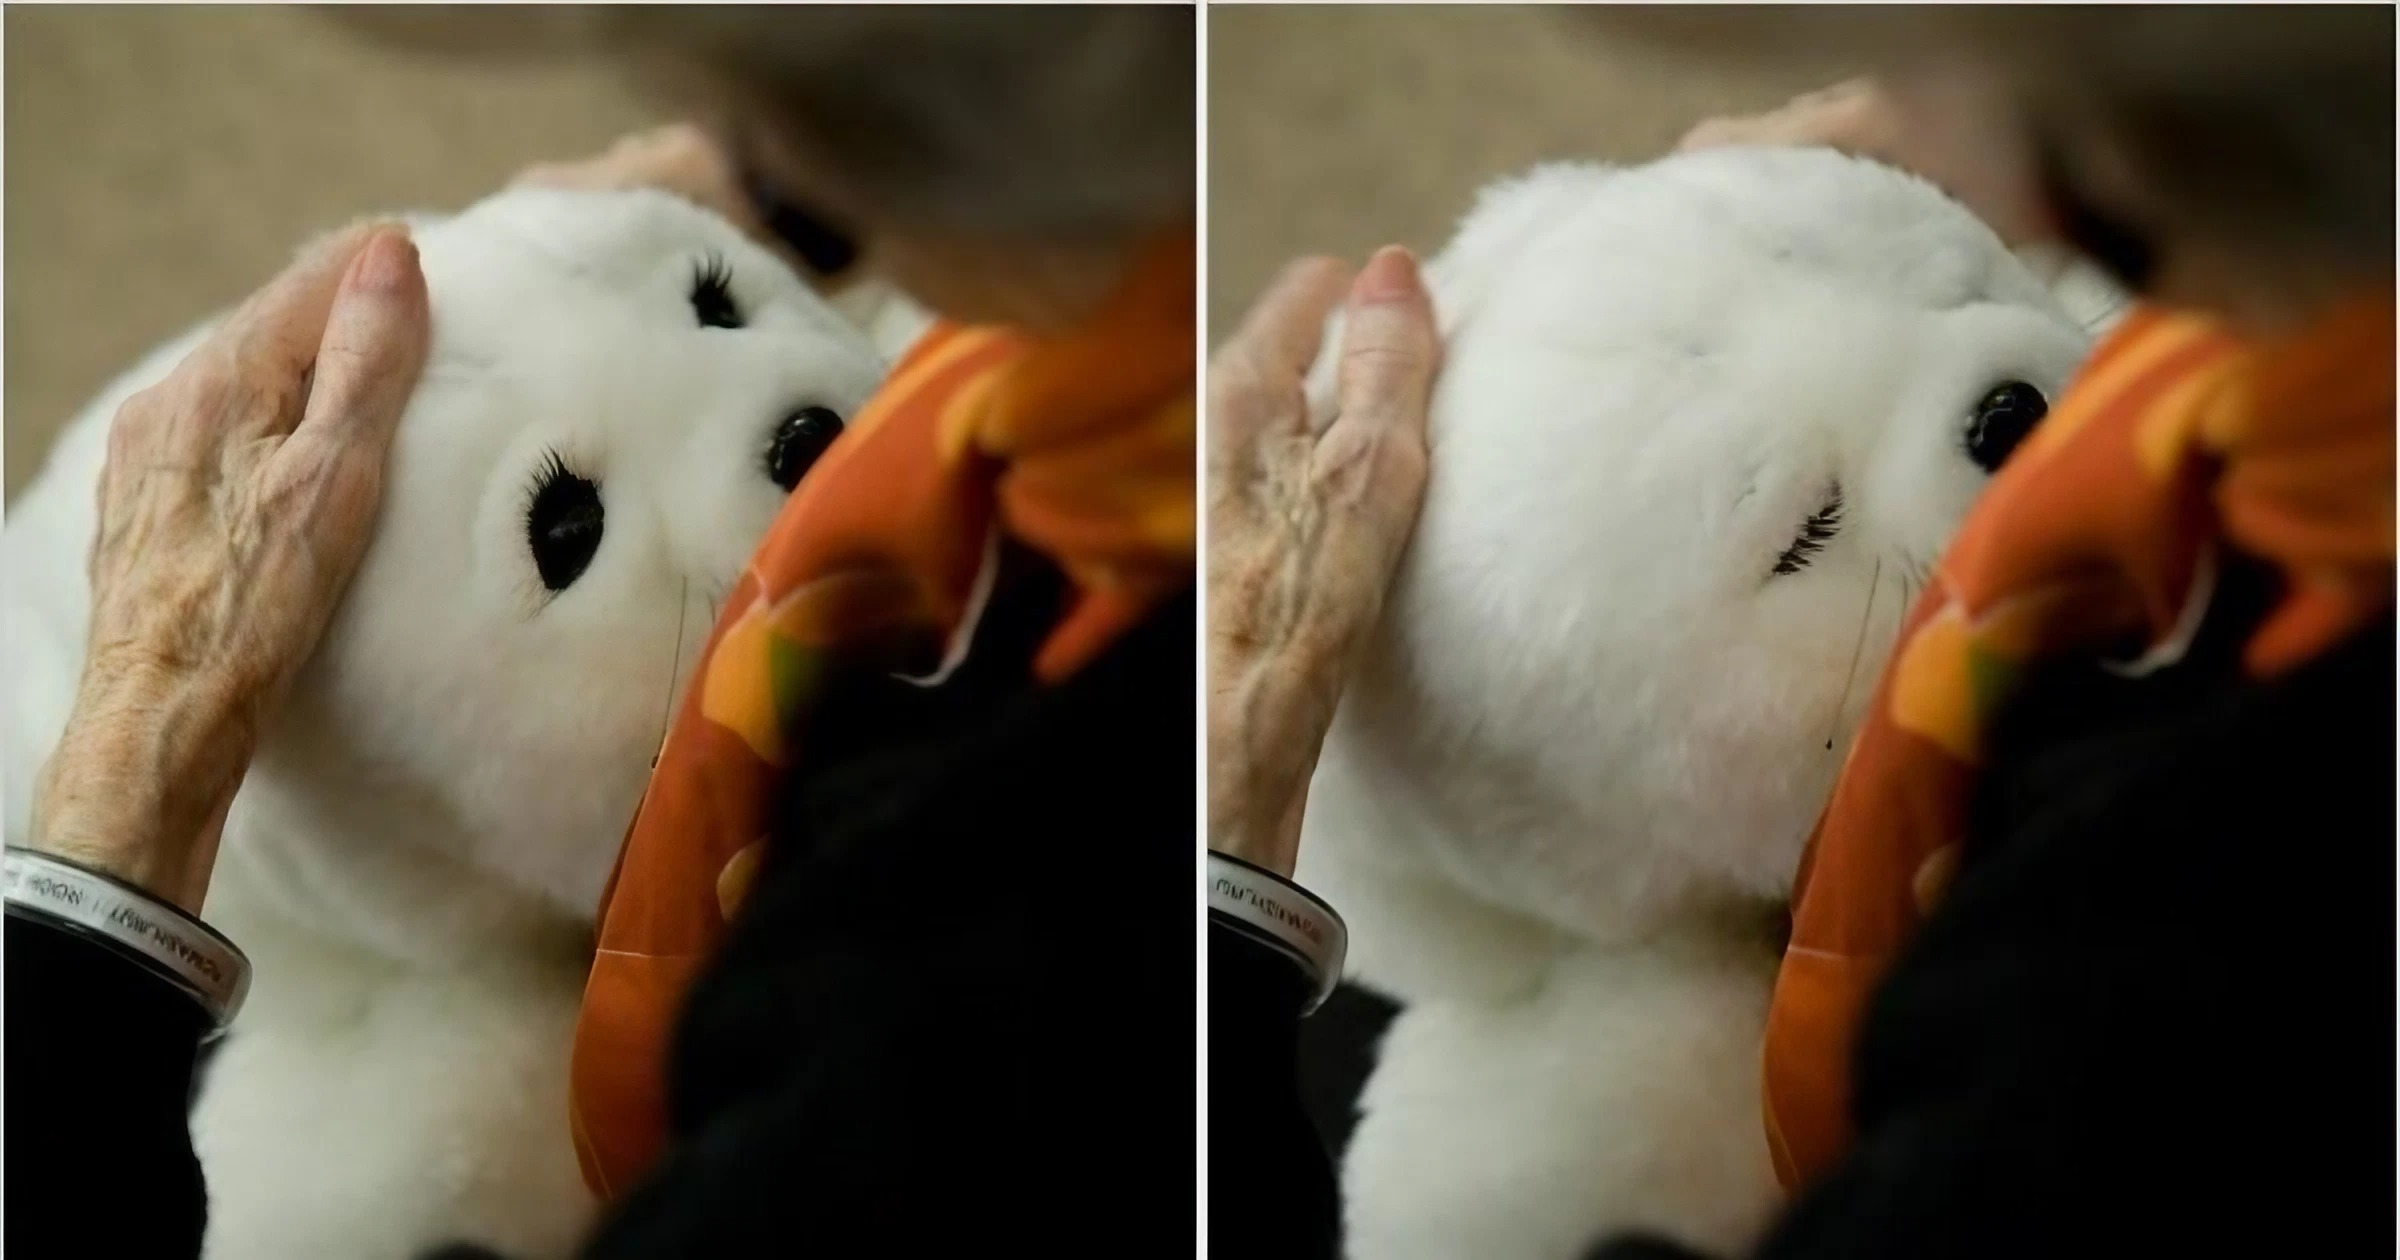
\includegraphics[width=0.4\linewidth]{figs/paro.jpeg}}
  \caption{Robots de entretenimiento}
\end{figure}

\subsubsection{Robots en salud}
Los robots en el campo de la salud están diseñados para proporcionar ayuda en entornos médicos y de atención sanitaria. Desempeñan tareas 
variadas como pueden ser la cirujía \ref{fig:davinci}, la rehabilitación \ref{fig:rehabilitacion} y la trasferencia de pacientes \ref{fig:trasferencia}, entre otros.

\begin{figure} [ht!]
  \centering    
  \subfigure[Da Vinci]{\label{fig:davinci}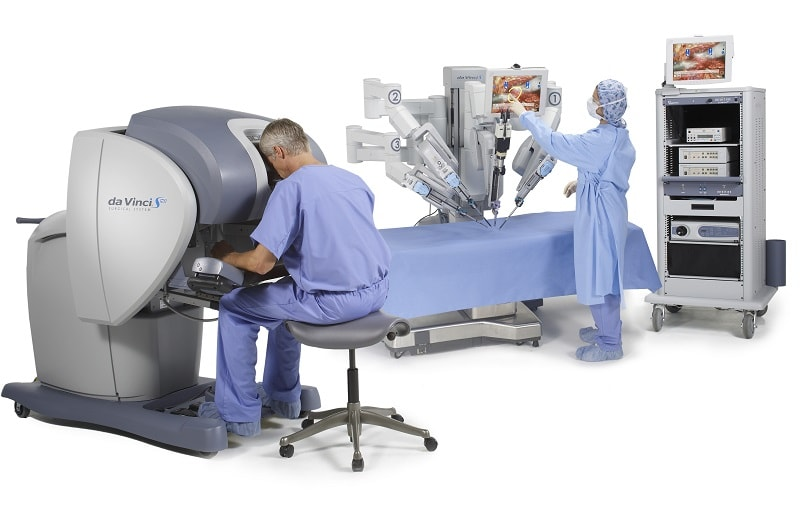
\includegraphics[width=0.35\linewidth ]{figs/davinci.jpg}}
  \hspace{1cm}
  \subfigure[Atlas Marsi Bionics]{\label{fig:rehabilitacion}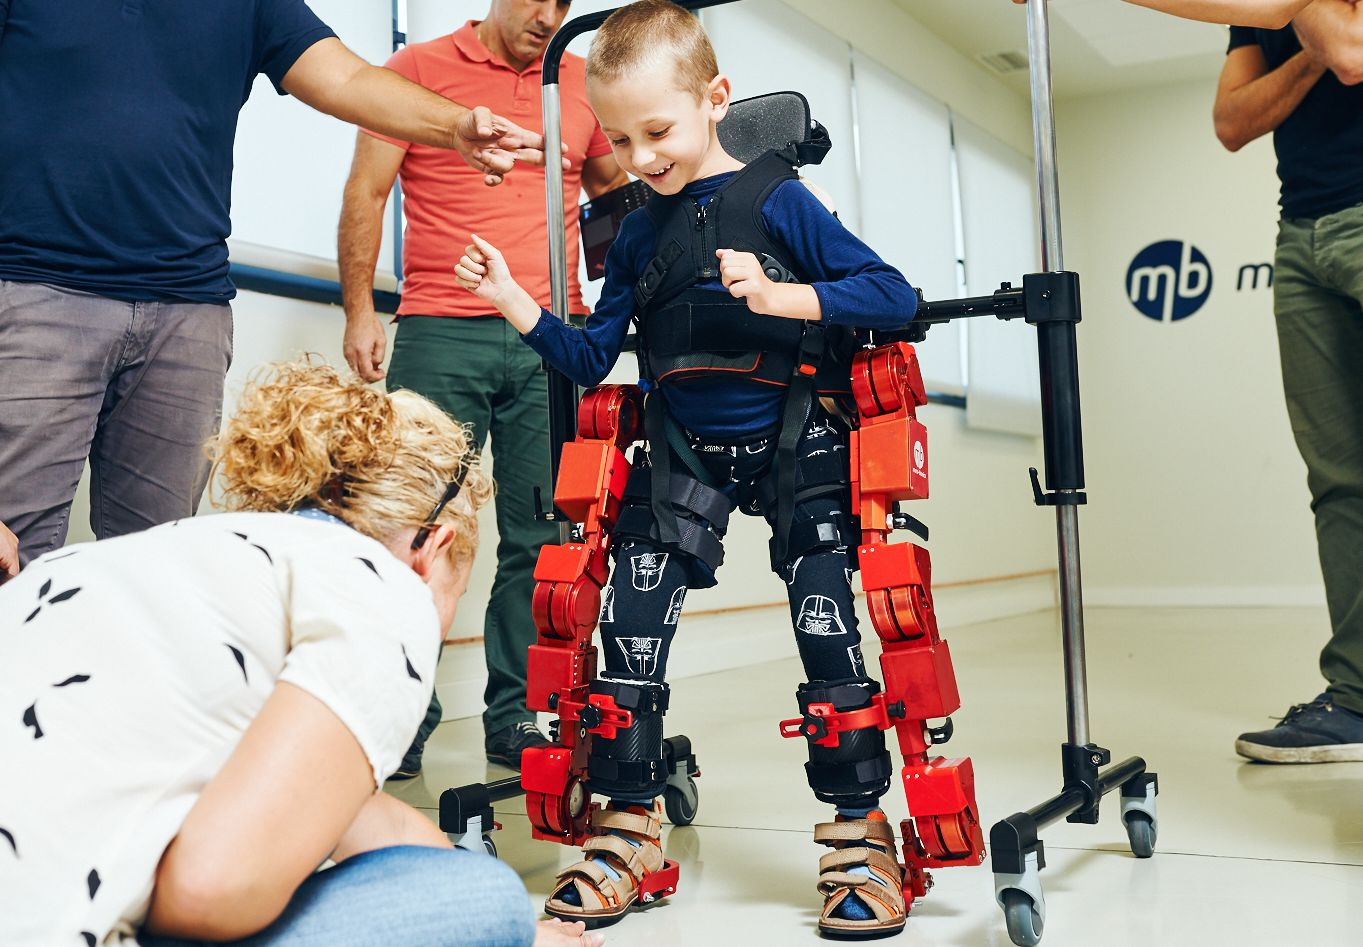
\includegraphics[width=0.35\linewidth]{figs/rehabilitacion.jpg}}
  \hspace{1cm}
  \subfigure[Riba 2]{\label{fig:trasferencia}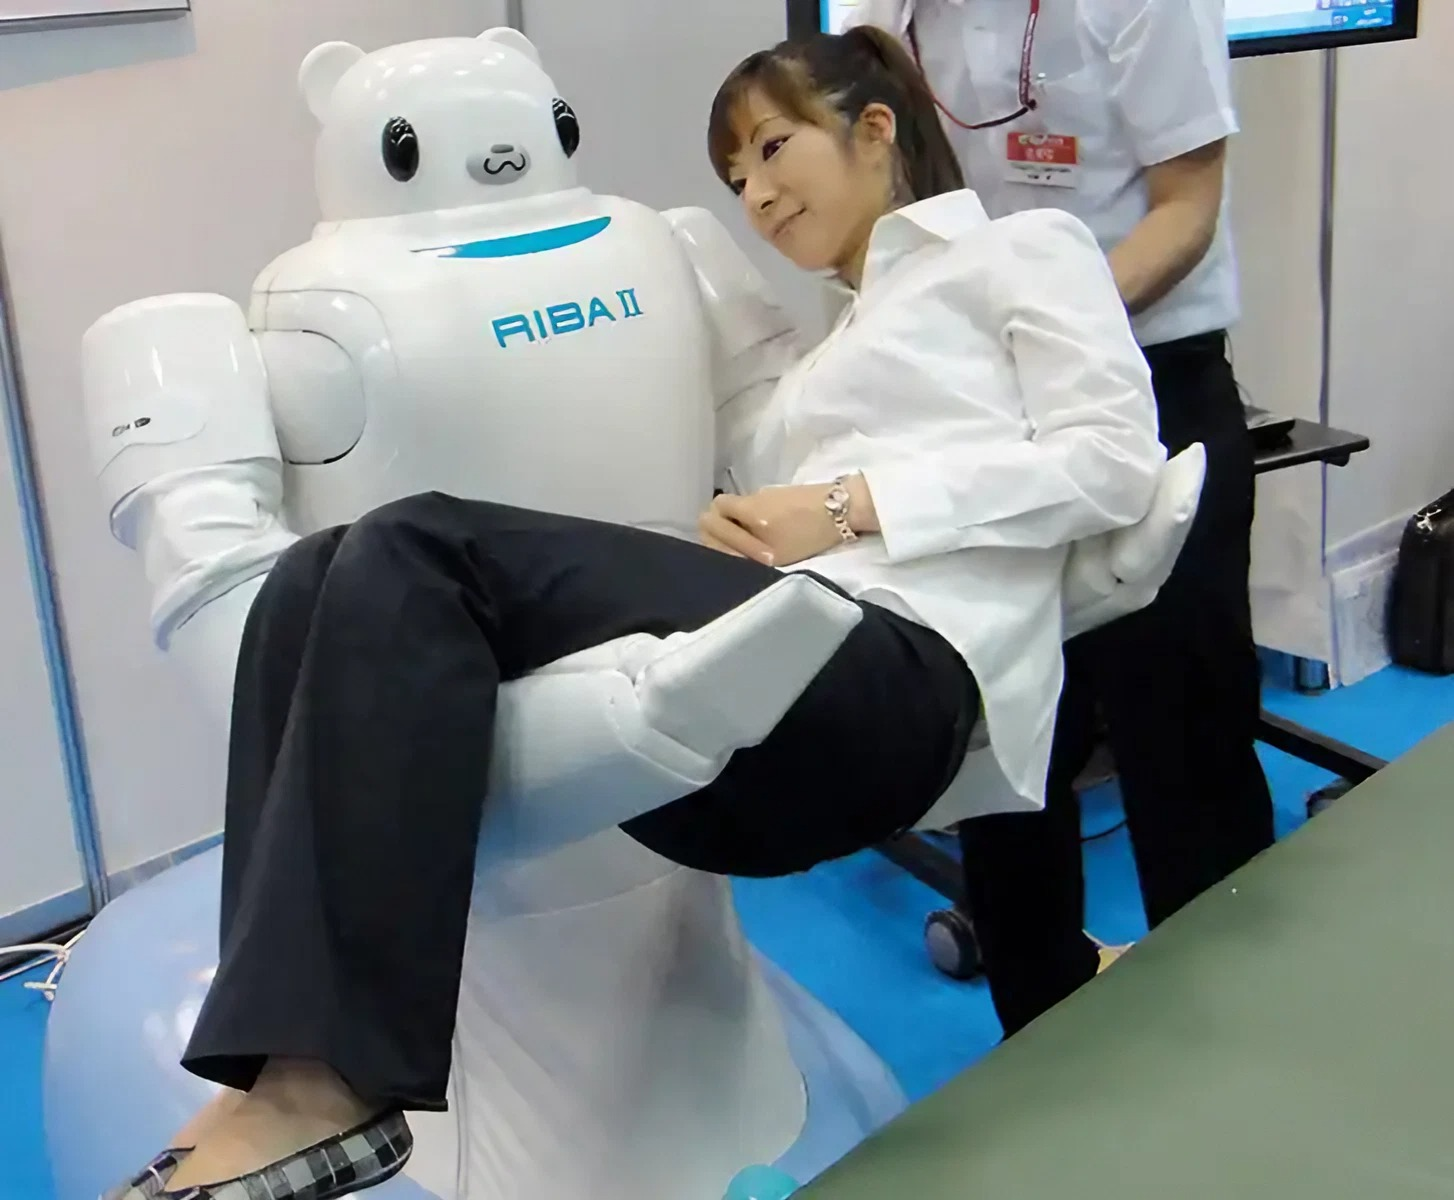
\includegraphics[width=0.35\linewidth]{figs/trasferencia.jpg}}
  \caption{Robots en el campo de la salud}
\end{figure}


\subsubsection{Robots en logística}
Los robots de logística están enfocados a tareas de trasporte y organización de mercancías en almacenes y centros de distribución. 
Son capaces de moverse de manera autónoma, cargar y descargar objetos ágilmente y bajo demanda optimizando los procesos logísticos. 
\\Los robots de logística destinados a usarse en almacenes pueden ser clasificados en 2 categorías:
\begin{itemize}
\item \ac{AGV}: Son robots filoguiados, es decir, solo se pueden desplazar a lo largo de un carril preestablecido. Este carril puede ser 
una línea pintada en el suelo o un riel metálico. Son baratos pero son poco flexibles.
\item \ac{AMR}: Son la evolución de los \acs{AGV}. Están dotados con una gran variedad de sensores para poder auto-localizarse y 
detectar obstáculos. Son capaces de navegar autonomamente transportando cargas pesadas, como \textit{palets} o estanterías, en colaboración 
con el resto de la flota. Además son adaptables y fáciles de desplegar pero su coste es más elevado.
\end{itemize}

\begin{figure} [ht!]
    \centering    
    \subfigure[AGV Linde C-MATIC \footnote{\url{https://www.linde-mh.es/es/Productos/Carretillas-automatizadas/C-MATIC/}}]{\label{fig:agv}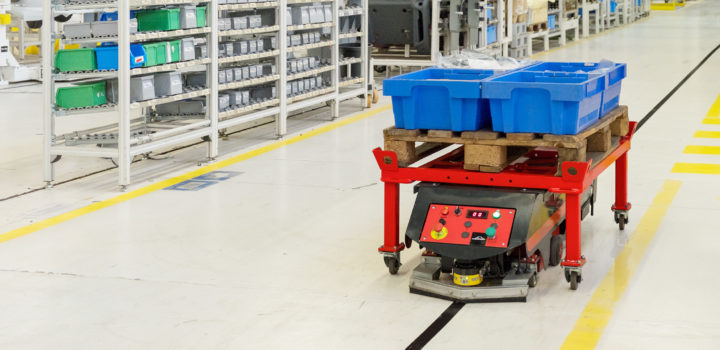
\includegraphics[width=0.4\linewidth ]{figs/agv.jpg}}
    \hspace{1cm}
    \subfigure[AMR Amazon Robotics]{\label{fig:amr}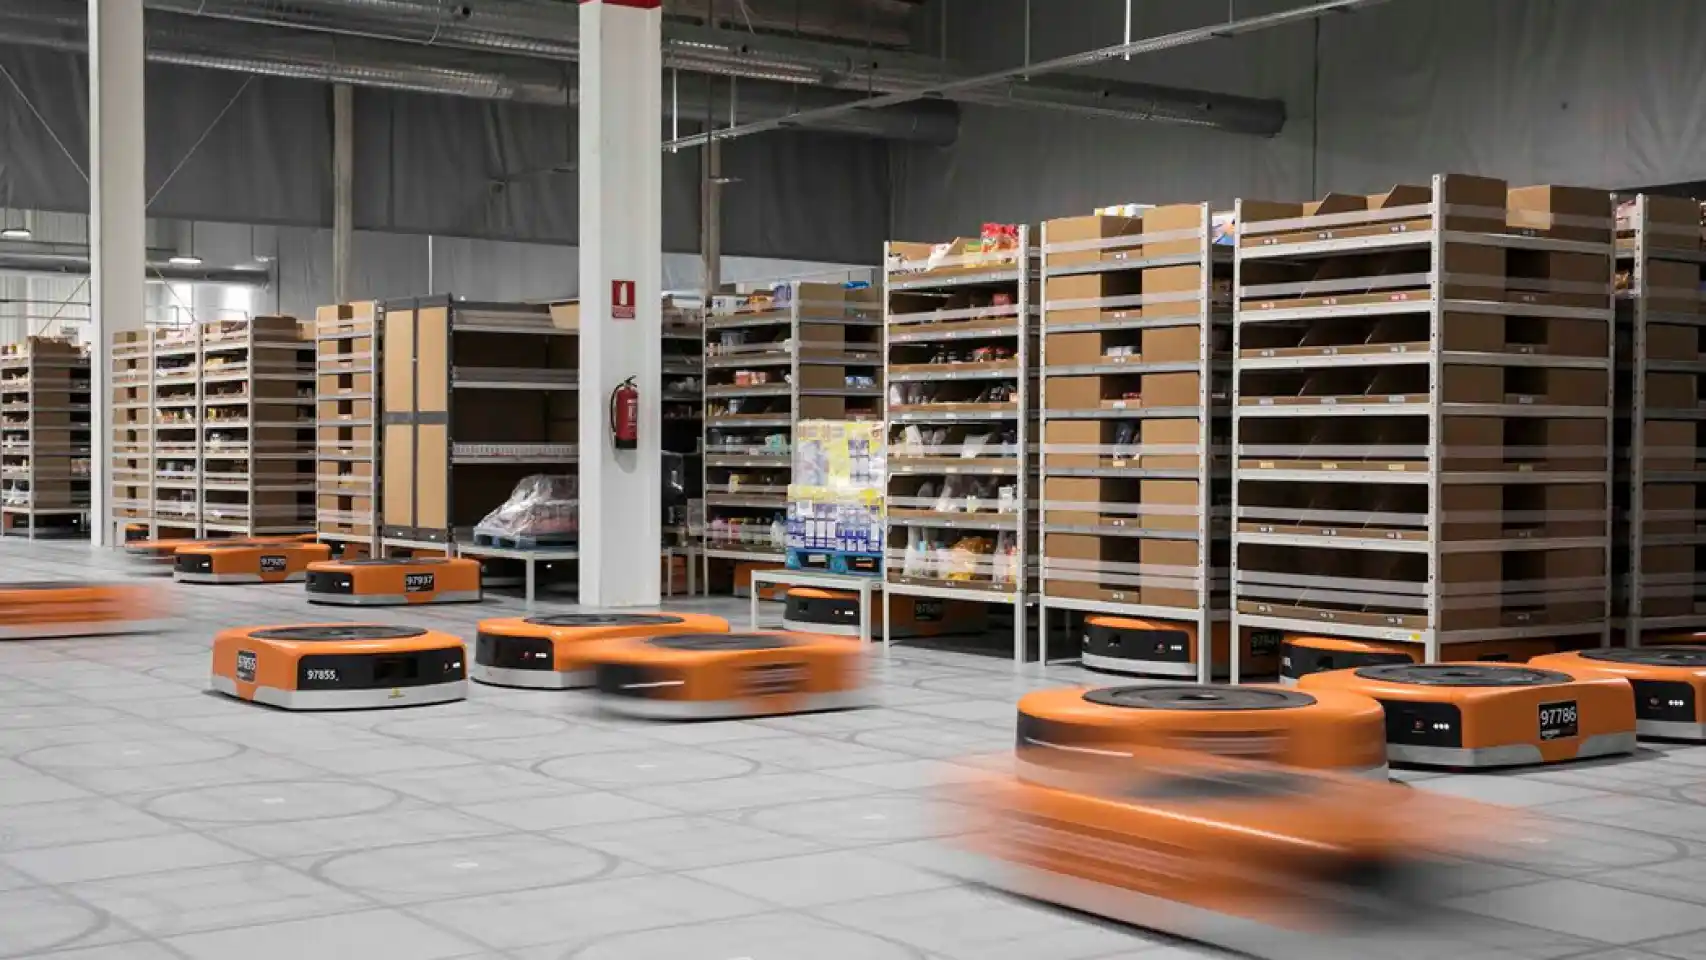
\includegraphics[width=0.4\linewidth]{figs/amr.jpg}}
    \caption{Robots de logística usados en almacenes}
\end{figure}

Más allá de su uso de almacenes, cabe destacar los llamados robots de "última milla". Son aquellos usados en el reparto de comida y 
paquetes en las ciudades. Aunque actualmente se encuentra en fase de desarrollo, ya ha sido probados algunos 
prototipos como el usado por Glovo en Londres para repartir comida.
\begin{figure} [ht!]
    \begin{center}
      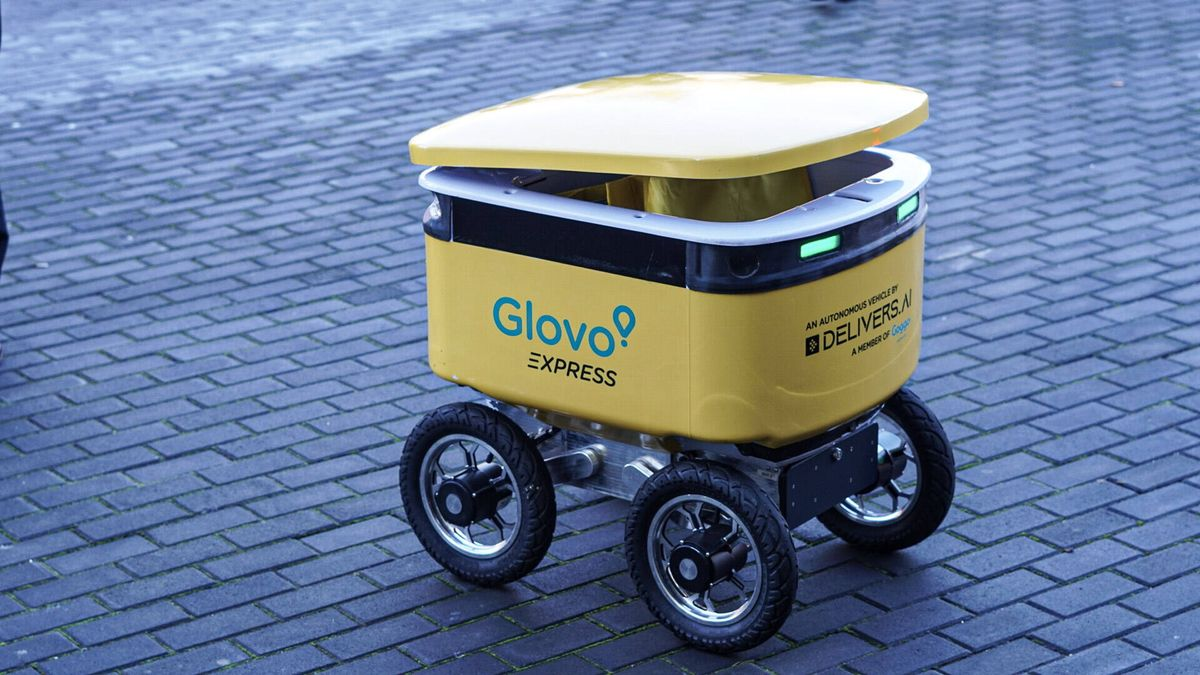
\includegraphics[width=8cm]{figs/reparto.jpg}
    \end{center}
    \caption{Robot de reparto de Glovo}
    \label{fig:glovo}
\end{figure}\ 

\newpage
\subsection{Robótica industrial}
\label{sec:rob_industrial}
Se entiende por robot industrial a una máquina automatizada diseñada específicamente para llevar a cabo tareas en entornos industriales. 
Disponen de numerosas articulaciones y una gran capacidad de maniobrabilidad. Su objetivo principal es remplazar a un 
operario humano en tareas aburridas, sucias, peligrosas y exigentes (\textit{4D: Dull, Dirty, Dangerous and Demanding}).
En función de el número de articulaciones y la geometría del manipulador, se pueden clasificar en diferentes categorías.

\subsubsection{SCARA}
Los robots de tipo \acs{SCARA} se caracterizan por la disposición de sus 4 articulaciones con todos los ejes de rotación perpendiculares al suelo. Su capacidad para 
realizar movimientos rápidos y precisos en un plano horizontal lo hacen ideal para su uso en aplicaciones de ensamblaje electrónico, operaciones de 
\textit{pick and place} (coger componentes y situarlos) y empaquetado de productos, entre otras.
\begin{figure} [h!]
  \centering    
  \subfigure[Ensamblado de baterías]{\label{fig:fanuc}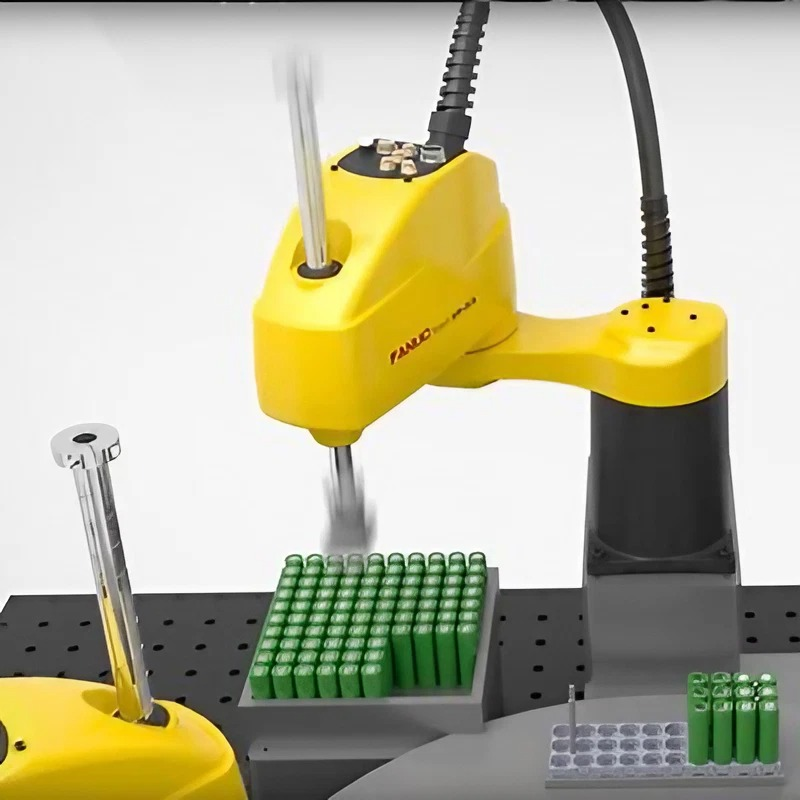
\includegraphics[width=0.3\linewidth ]{figs/fanuc.jpg}}
  \hspace{3cm}
  \subfigure[Espacio de trabajo]{\label{fig:fanuc_ws}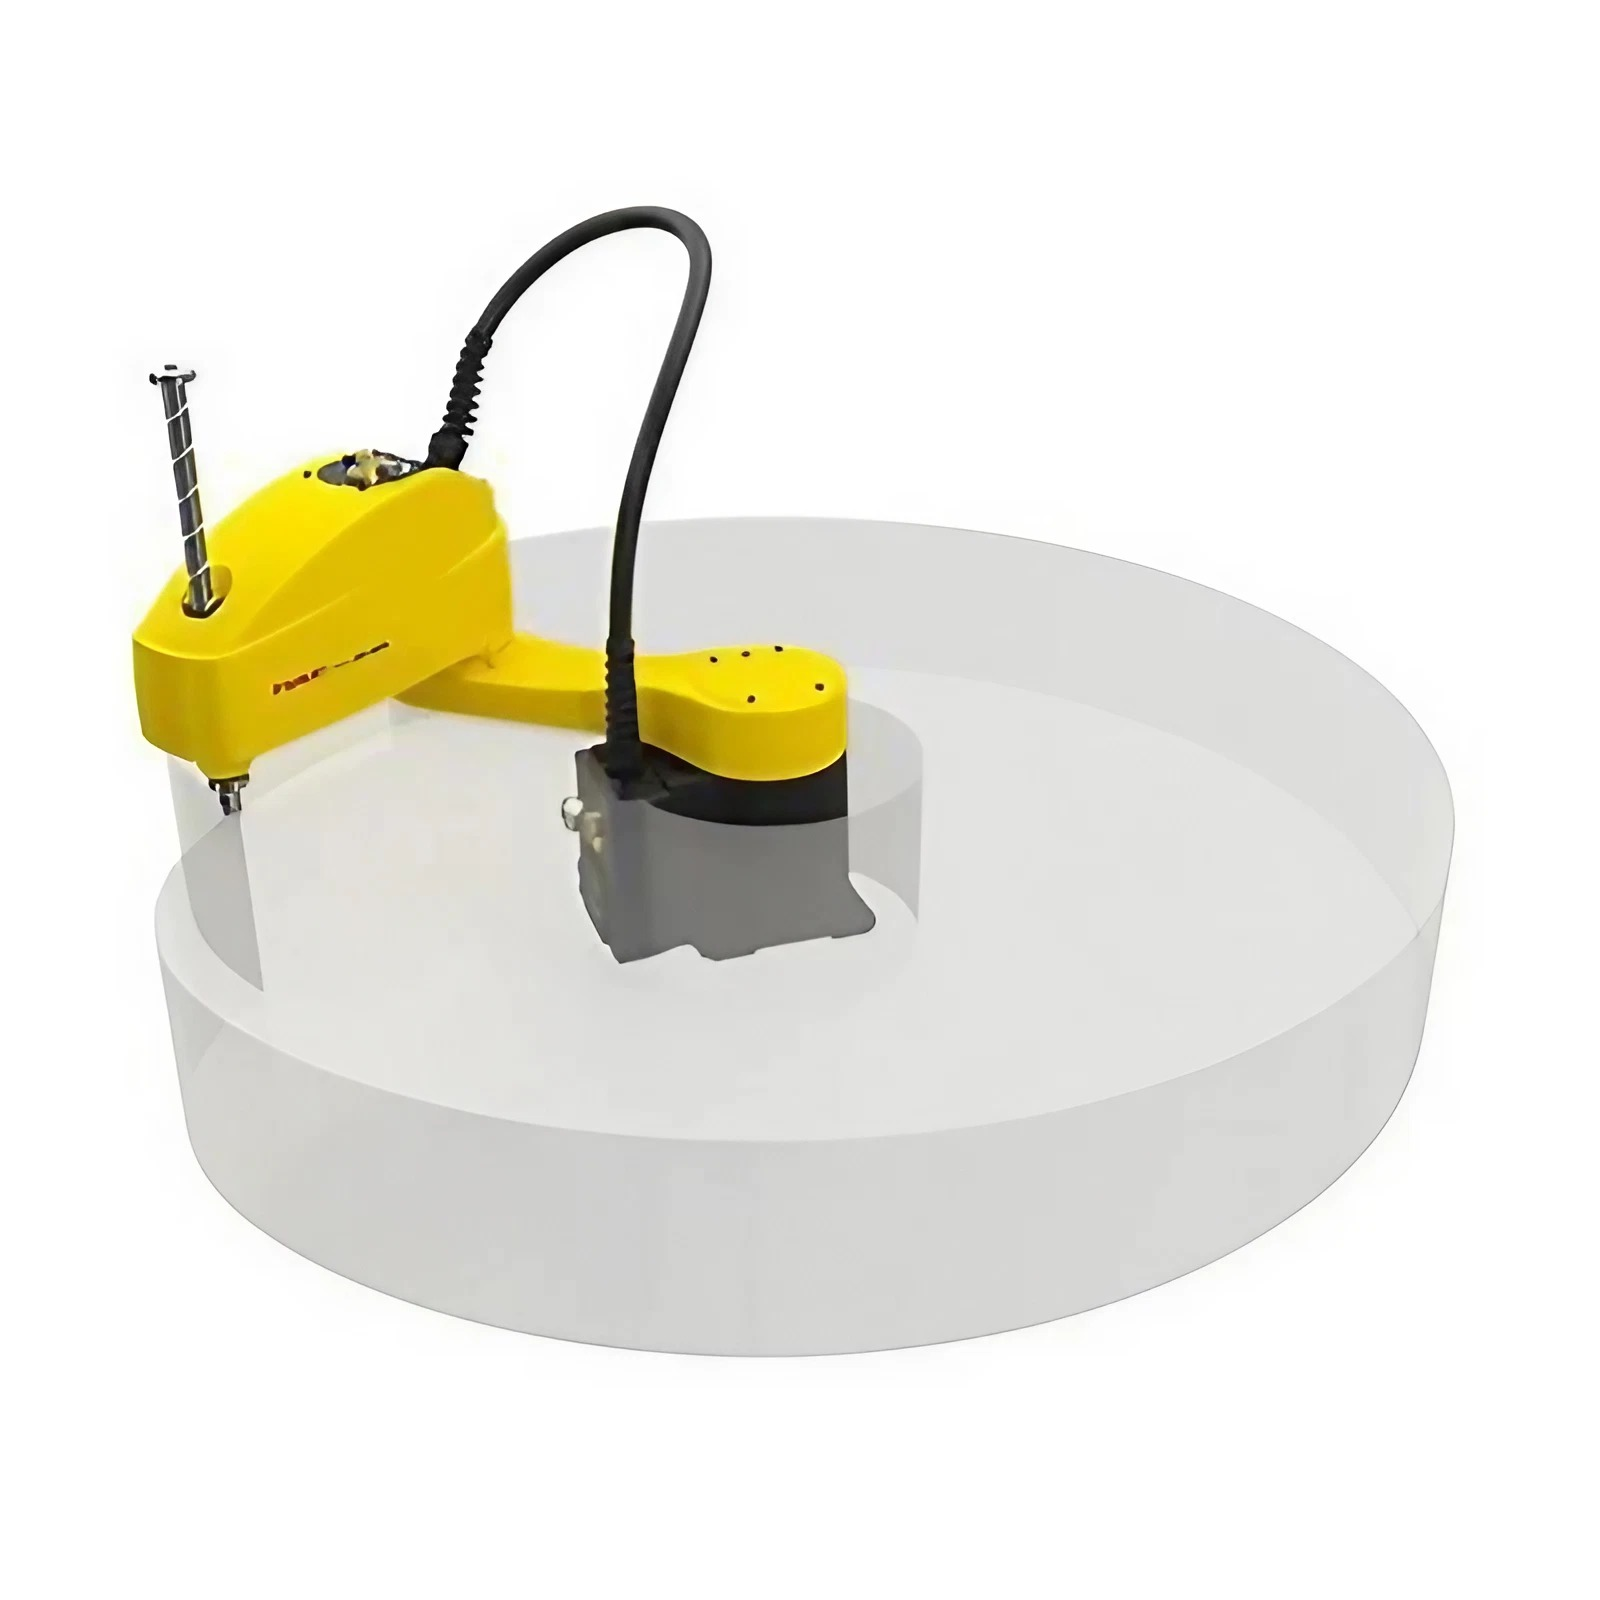
\includegraphics[width=0.4\linewidth]{figs/fanuc_spacio.jpg}}
  \caption[Fanuc SR-3iA]{Ejemplo: FANUC SR-3iA \footnote{\url{https://www.fanuc.eu/uk/en/robots/robot-filter-page/scara-series/scara-sr-3ia}}}
\end{figure}
\newpage
\subsubsection{Articulados}
Es el tipo de brazo robótico más usado en la industria. Están formados por una estructura similar a la de un brazo humano. Poseen entre 4 y 6 articulaciones de tipo 
revolución (giran en torno a un eje) permitiendo realizar movimientos complejos. 
\begin{figure} [h!]
  \centering    
  \subfigure[KUKA IONTEC \footnote{\url{https://www.kuka.com/es-es/productos-servicios/sistemas-de-robot/robot-industrial/kr-iontec}}]{\label{fig:iontec}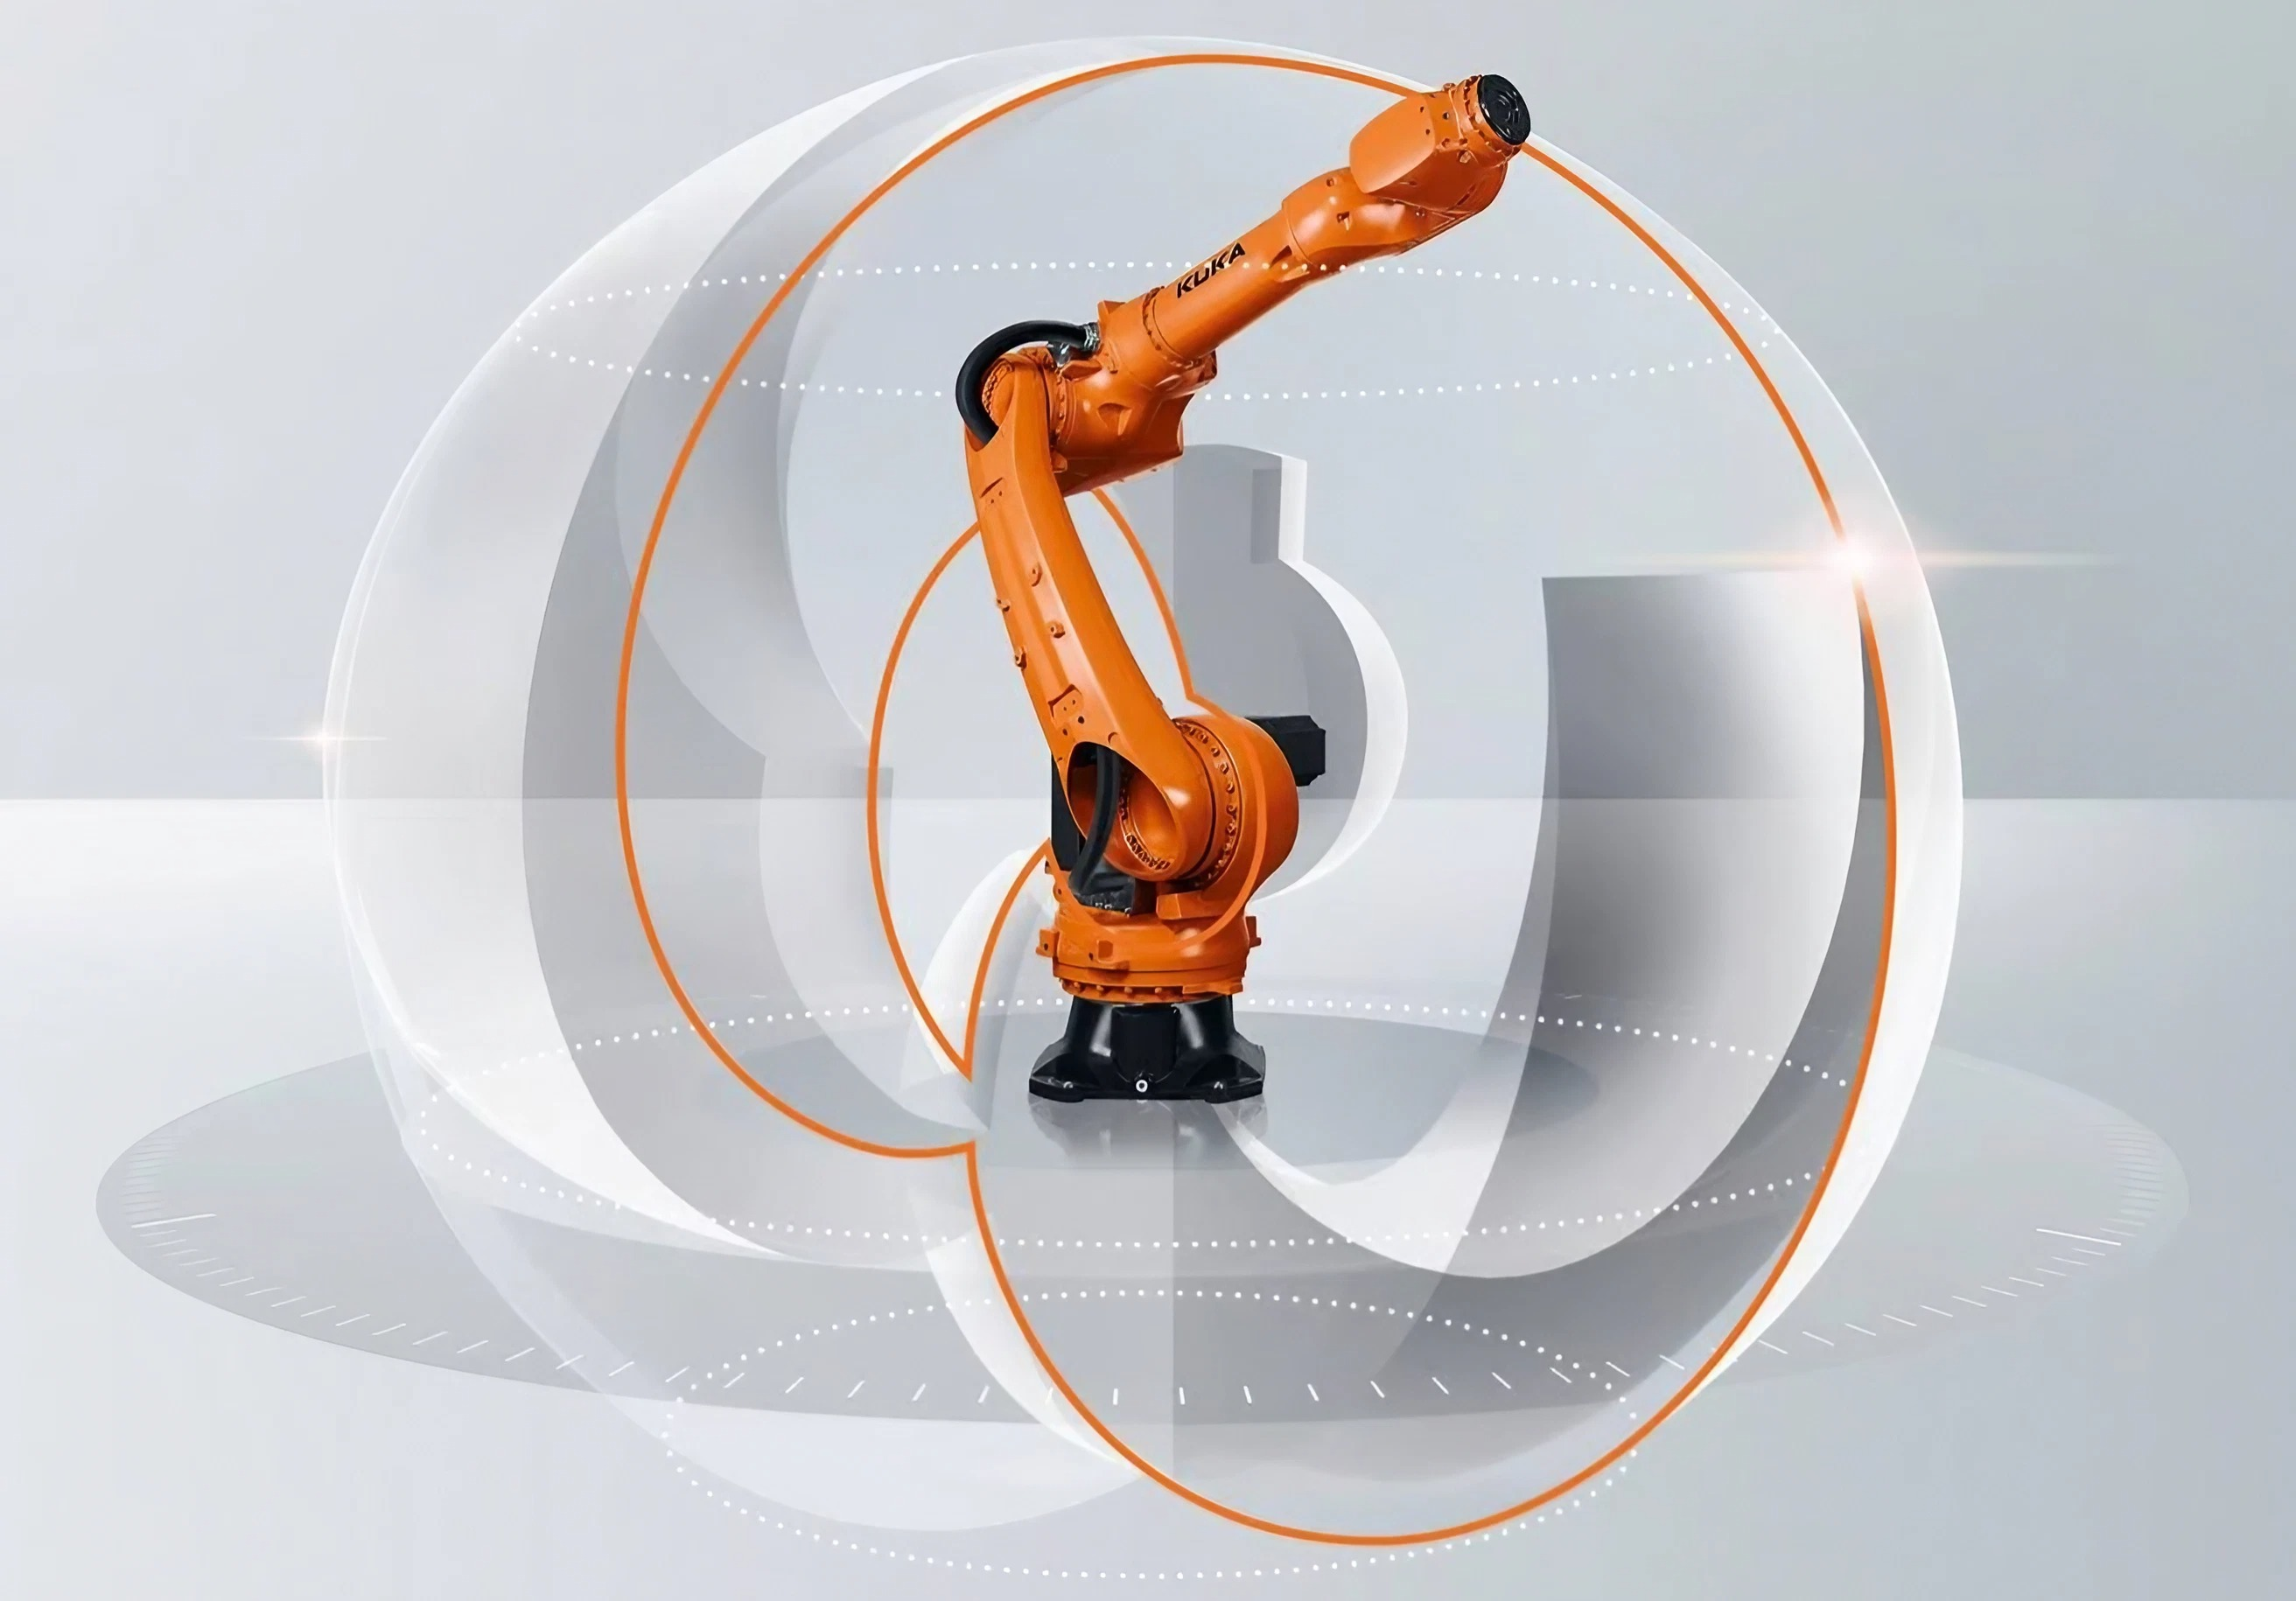
\includegraphics[width=0.4\linewidth ]{figs/kuka_articulado.jpg}}
  \hspace{1.5cm}
  \subfigure[ABB IRB 6700 \footnote{\url{https://new.abb.com/products/robotics/robots/articulated-robots/irb-6700}}]{\label{fig:irb6700}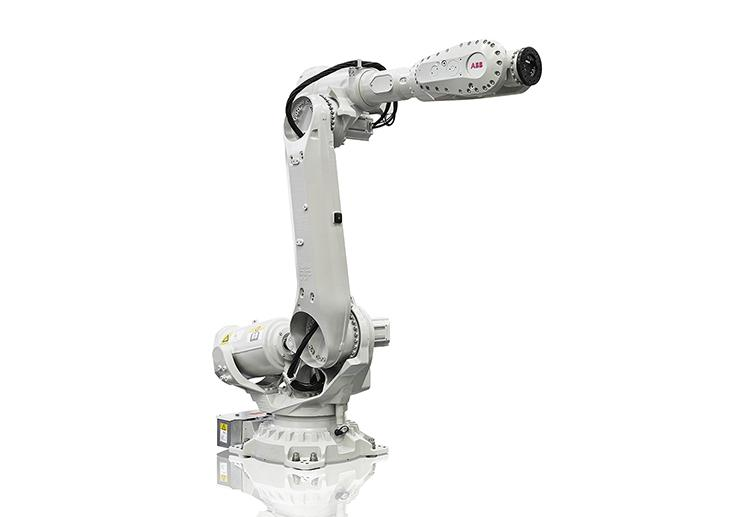
\includegraphics[width=0.4\linewidth]{figs/irb.jpg}}
  \caption{Robot articulados}
\end{figure}

\subsubsection{Paralelos}
Son un tipo de robot industrial que se caracteriza por tener una estructura mecánica en la cual varios brazos o cadenas cinemáticas se conectan de forma paralela a una plataforma móvil o 
base. Estos robots son rápidos y liviano, por lo que son ideales para aplicaciones que requieren alta velocidad, como en la industria alimentaria o en la selección y
empaquetado de productos.

\begin{figure} [ht!]
  \centering    
  \subfigure[Robot Delta ABB]{\label{fig:delta}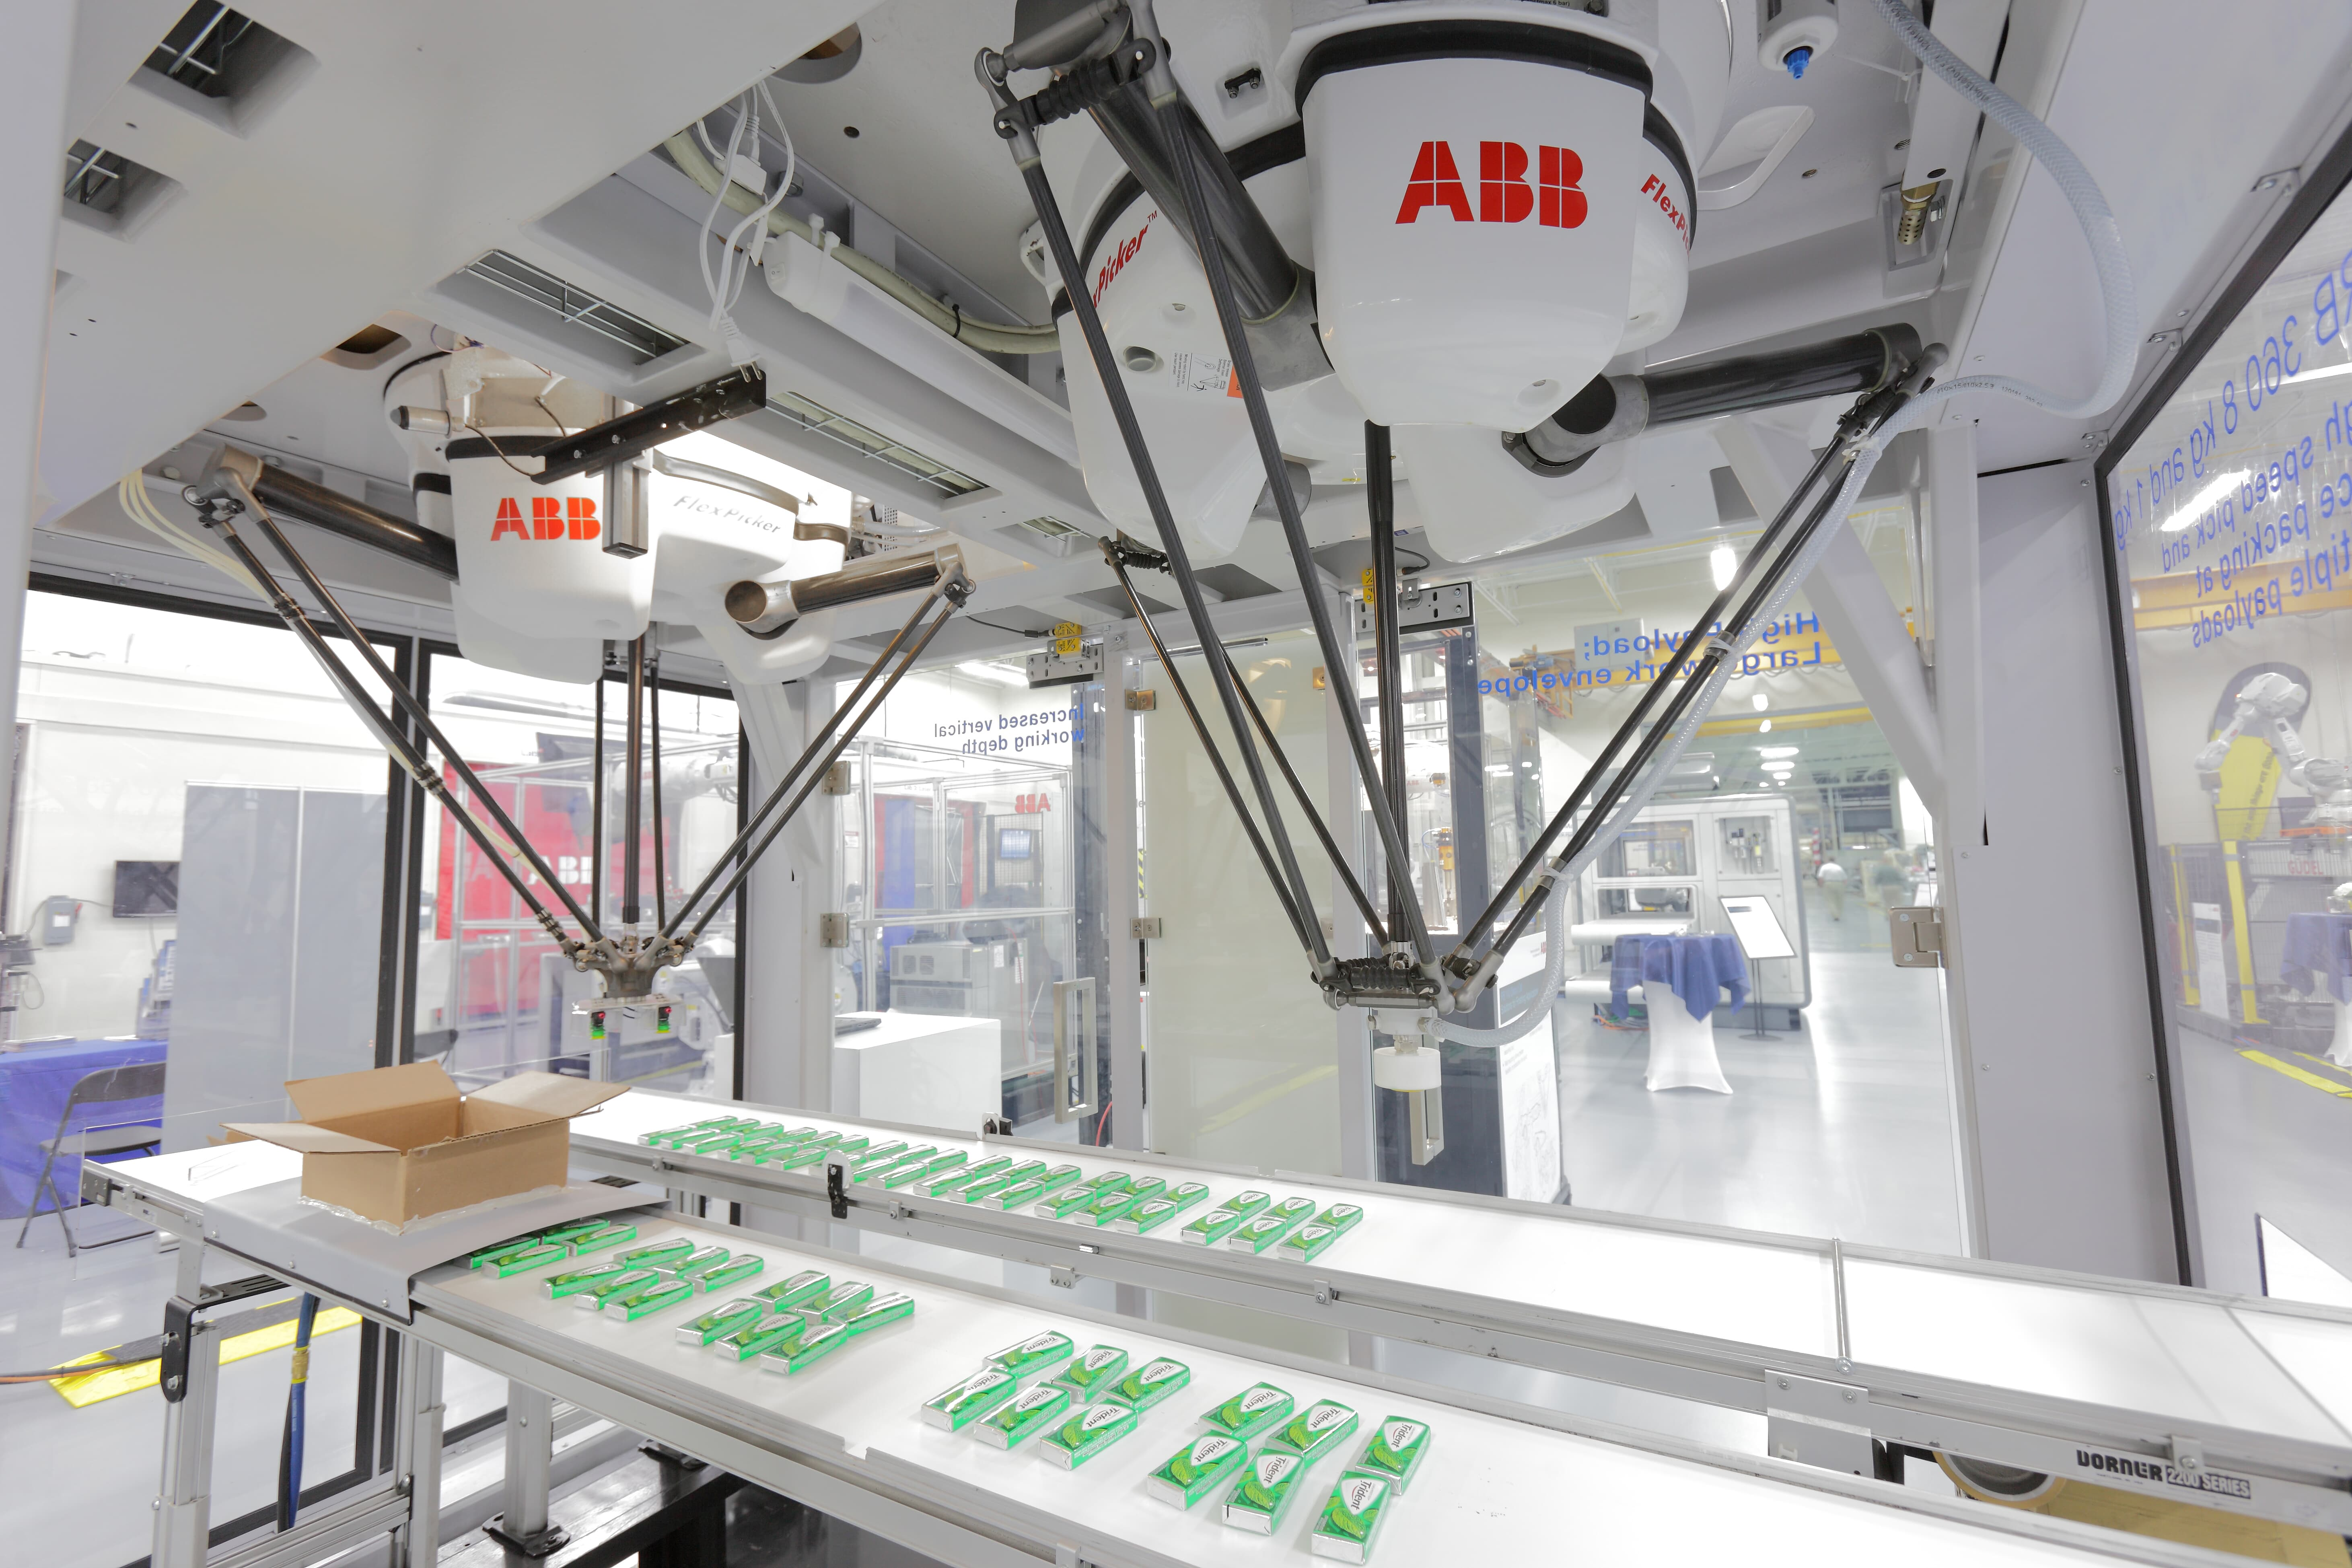
\includegraphics[width=0.4\linewidth ]{figs/delta_flex_picker.png}}
  \hspace{1cm}
  \subfigure[FANUC M-410iC]{\label{fig:paral}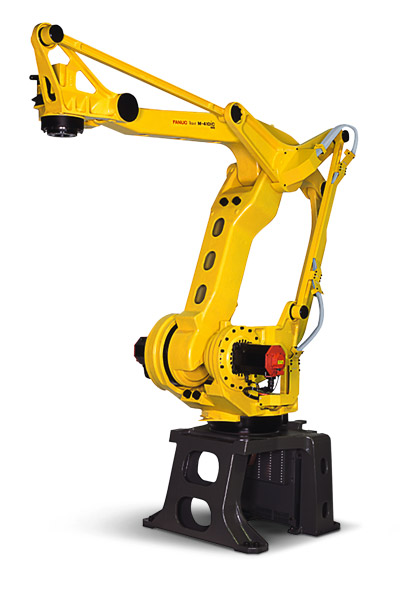
\includegraphics[width=0.4\linewidth]{figs/m_410.jpg}}
  \caption{Robots basados en paralelogramos}
\end{figure}

\newpage
\subsubsection{Cartesianos}
Los robots pertenecientes a esta categoría, se mueven a lo largo de unas guías lineales en la dirección de los tres ejes cartesianos (X, Y, Z) y cuyos ejes forman ángulos rectos entre sí. \\
Se trata de un tipo de máquina muy común en la industria y es usada en tareas de \textit{pick and place} y fresado, entre otras.

\begin{figure} [h!]
  \centering    
  \subfigure[VP-2500DP \footnote{\url{https://www.smallsmt.biz/bestueckungsautomat/}}]{\label{fig:pnp}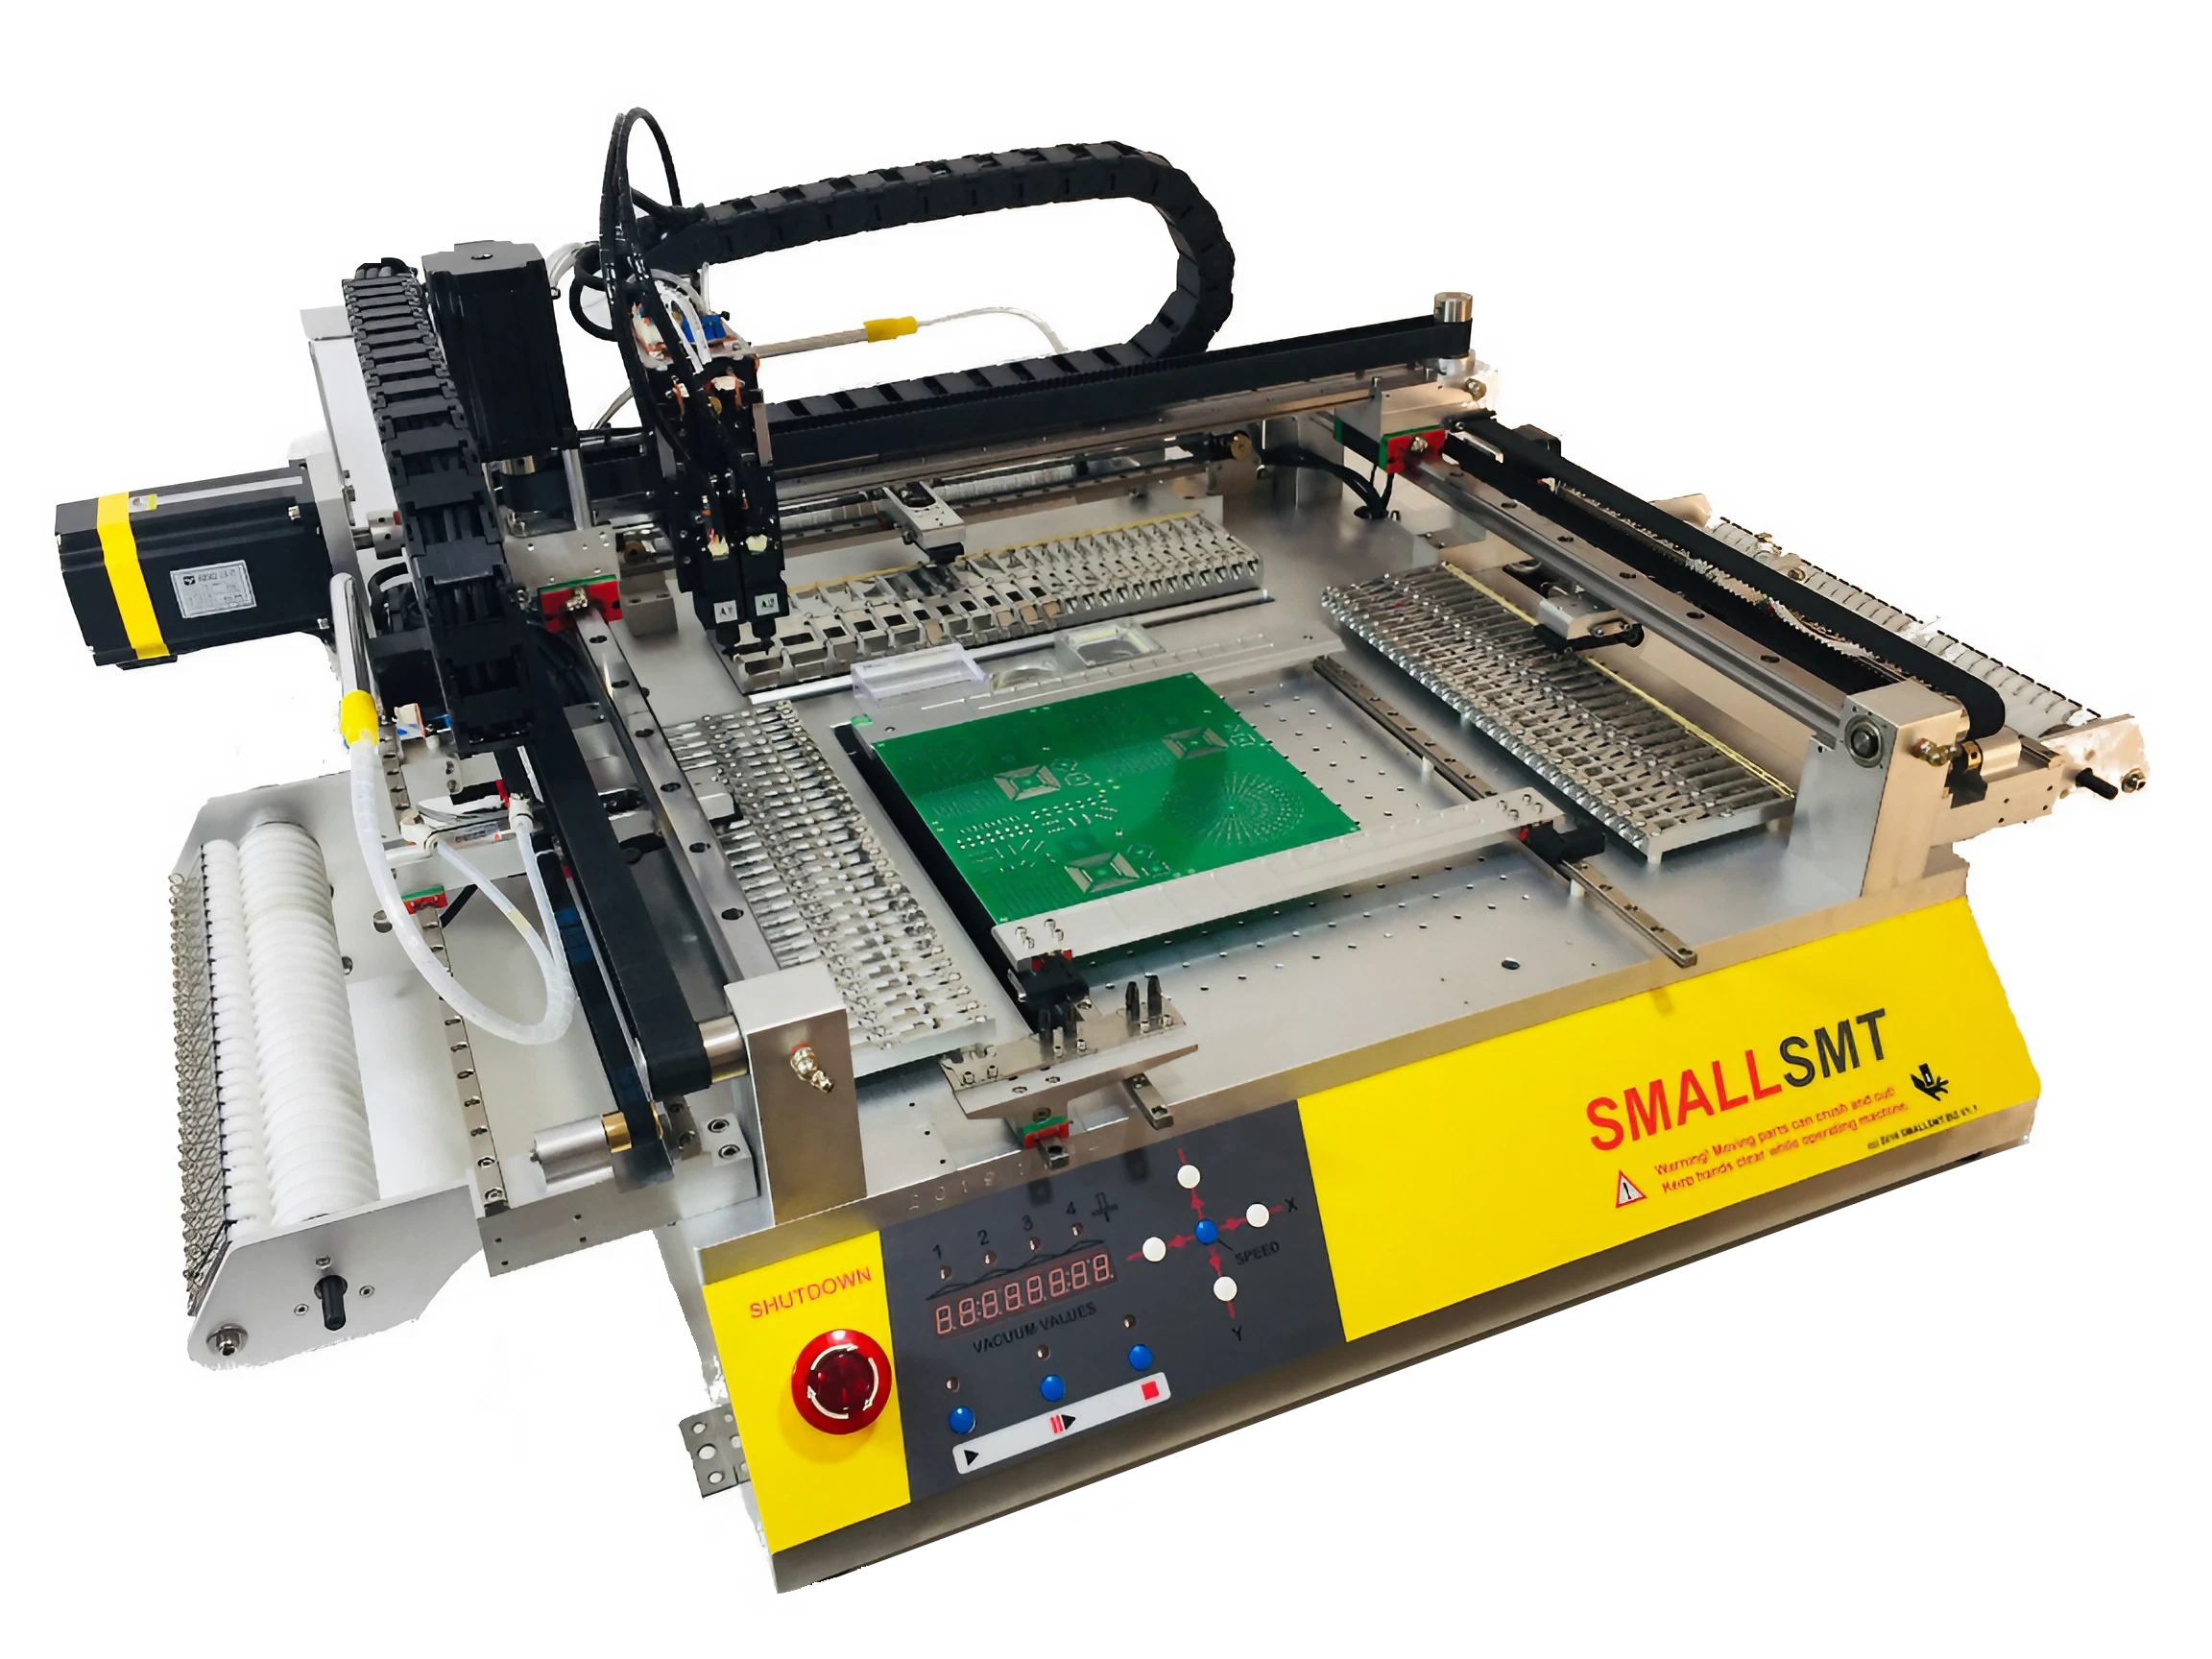
\includegraphics[width=0.4\linewidth ]{figs/pnp.jpg}}
  \hspace{1cm}
  \subfigure[OpenBuilds CNC Lead 1010 \footnote{\url{https://openbuilds.com/builds/lead-cnc-1010-40-x-40.7832/}}]{\label{fig:cnc}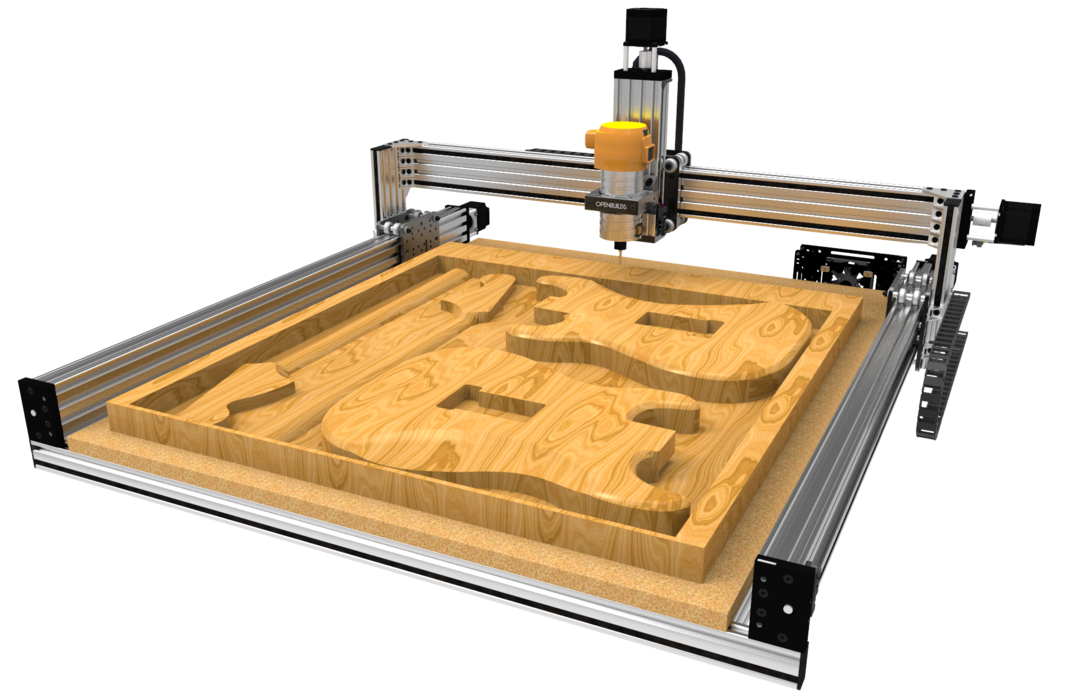
\includegraphics[width=0.4\linewidth]{figs/cnc.jpg}}
  \caption{Robots cartesianos}
\end{figure}

\section*{}
En resumen, la robótica es un campo en constante evolución que busca crear máquinas autónomas e inteligentes capaces de realizar una gran variedad de tareas cada vez 
más complejas.Sin embargo, a medida que la demanda de habilidades en robótica y automatización aumenta, se hace evidente la necesidad de formar a más personas en este campo.

\newpage
\section{Robótica educativa}
La robótica educativa es una disciplina que ha adquirido una gran relevancia en los últimos años debido a la creciente necesidad de formar a las nuevas generaciones en
competencias tecnológicas.

\label{sec:rob_educativa}
\subsection{Robótica en institutos}
En los institutos, se ha convertido en una herramienta pedagógica eficaz para desarrollar habilidades y conocimientos en áreas como la programación, 
la matemática, la electrónica y la resolución de problemas. Esto es conocido como \ac{STEM}. Gracias a esta formación, los 
estudiantes aprenden a diseñar, construir y programar robots simples para llevar a cabo una tarea específica, lo que les ayuda a comprender  
los conceptos de ciencia y tecnología de una manera más práctica e interactiva.\\
\begin{figure} [ht!]
  \centering    
  \subfigure[Instituto en Argentina \footnote{\url{https://www.diariodecuyo.com.ar/suplementos/Robotica-la-ciencia-de-aprender-jugando-20170907-0087.html}}]{\label{fig:instituto_sanjuan}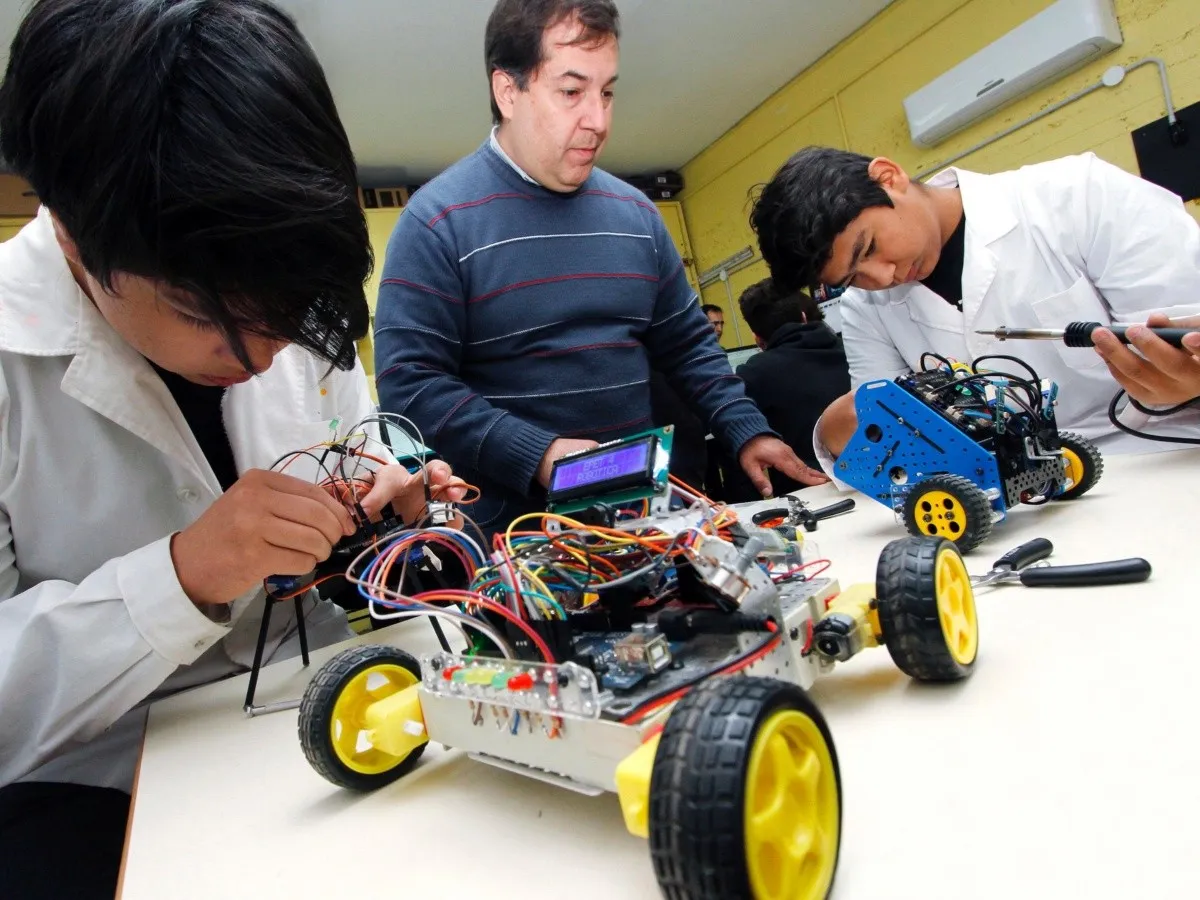
\includegraphics[width=0.4\linewidth ]{figs/robots_instituto.jpg}}
  \hspace{1cm}
  \subfigure[Institutos en Toledo \footnote{\url{https://www.uclmtv.uclm.es/institutos-de-camarena-y-madridejos-ganan-el-viii-torneo-de-robotica-organizado-por-la-uclm-en-toledo/}}]{\label{fig:instituto_toledo}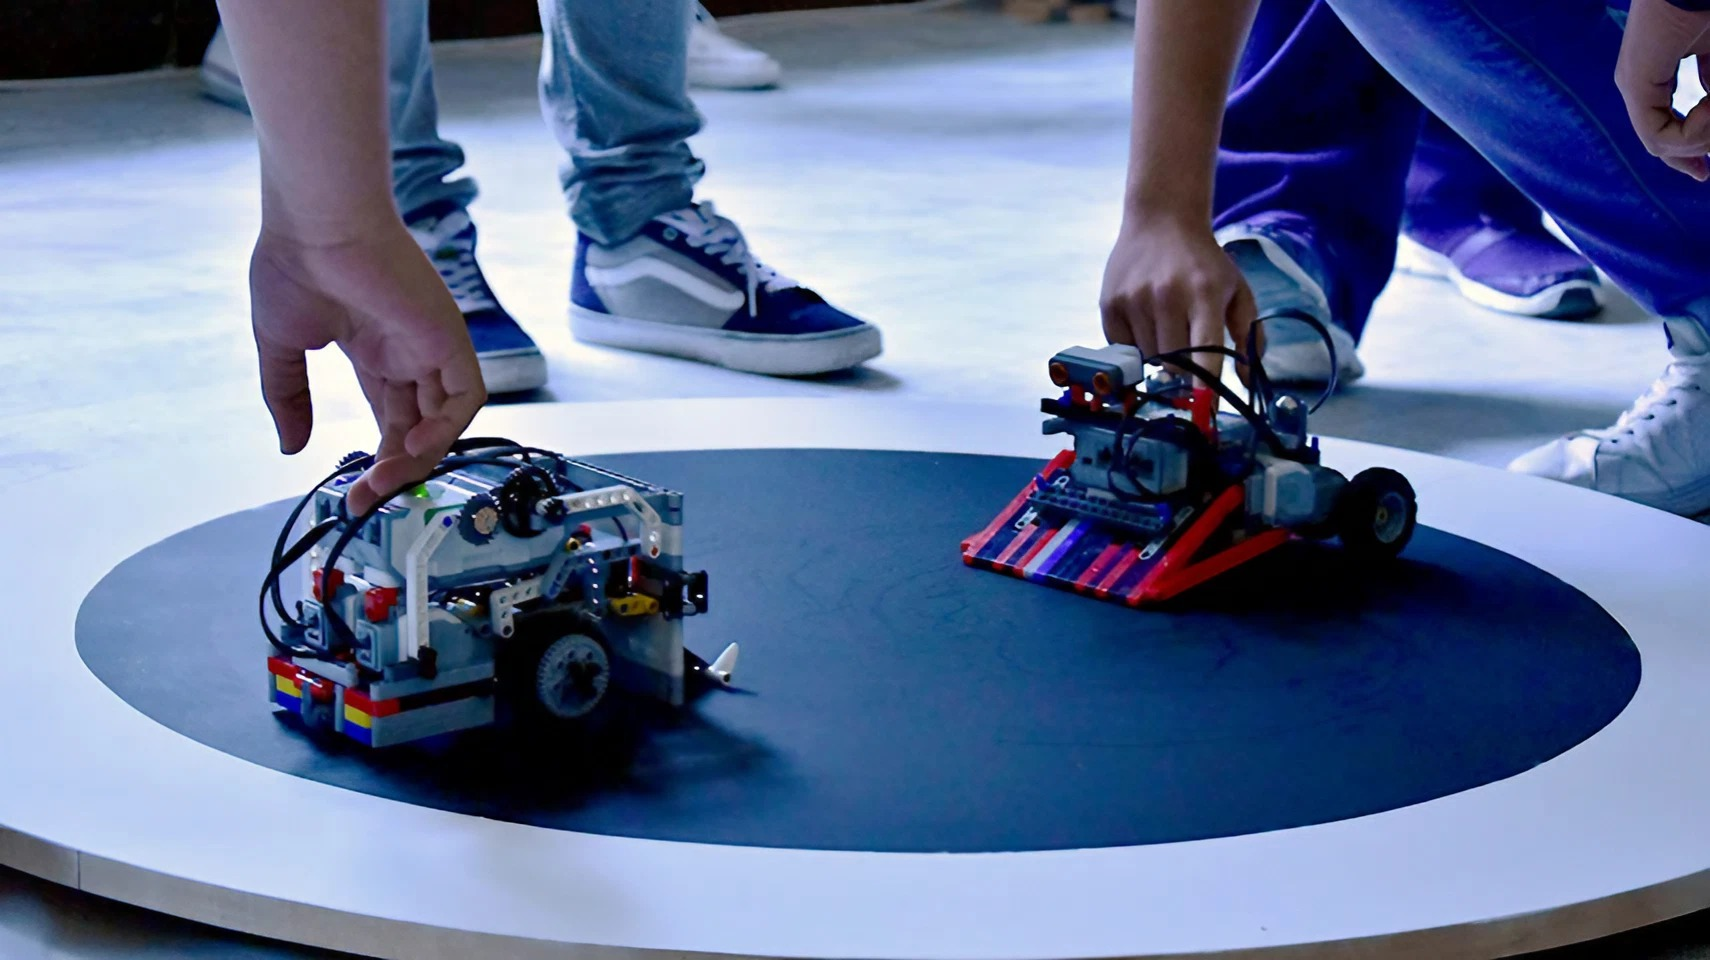
\includegraphics[width=0.5\linewidth]{figs/robot_batalla_instituto.jpg}}
  \caption{Robots en institutos}
\end{figure}

\newpage
\subsection{Robótica en universidades}
\begin{figure} [ht!]
  \centering    
  \subfigure[Kobuki Turtlebot 2 \footnote{\url{https://www.turtlebot.com/turtlebot2/}}]{\label{fig:turtlebot}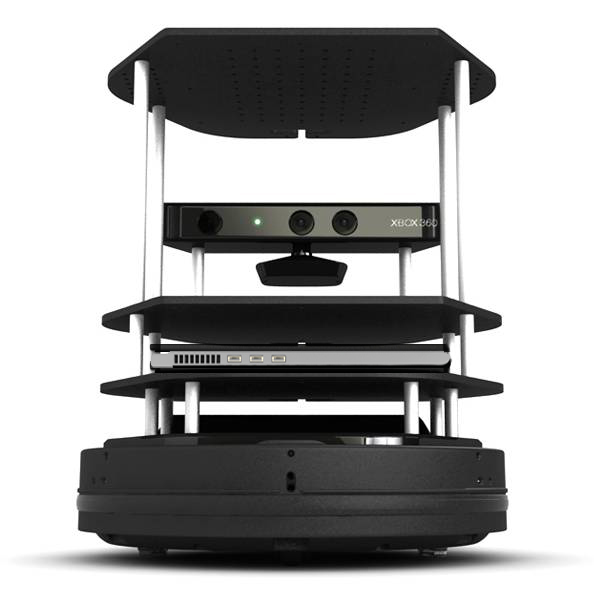
\includegraphics[width=0.4\linewidth ]{figs/turtlebot.jpg}}
  \hspace{1cm}
  \subfigure[Dobot Magician \footnote{\url{https://www.robotlab.com/store/dobot-robotic-arm}}]{\label{fig:dobot}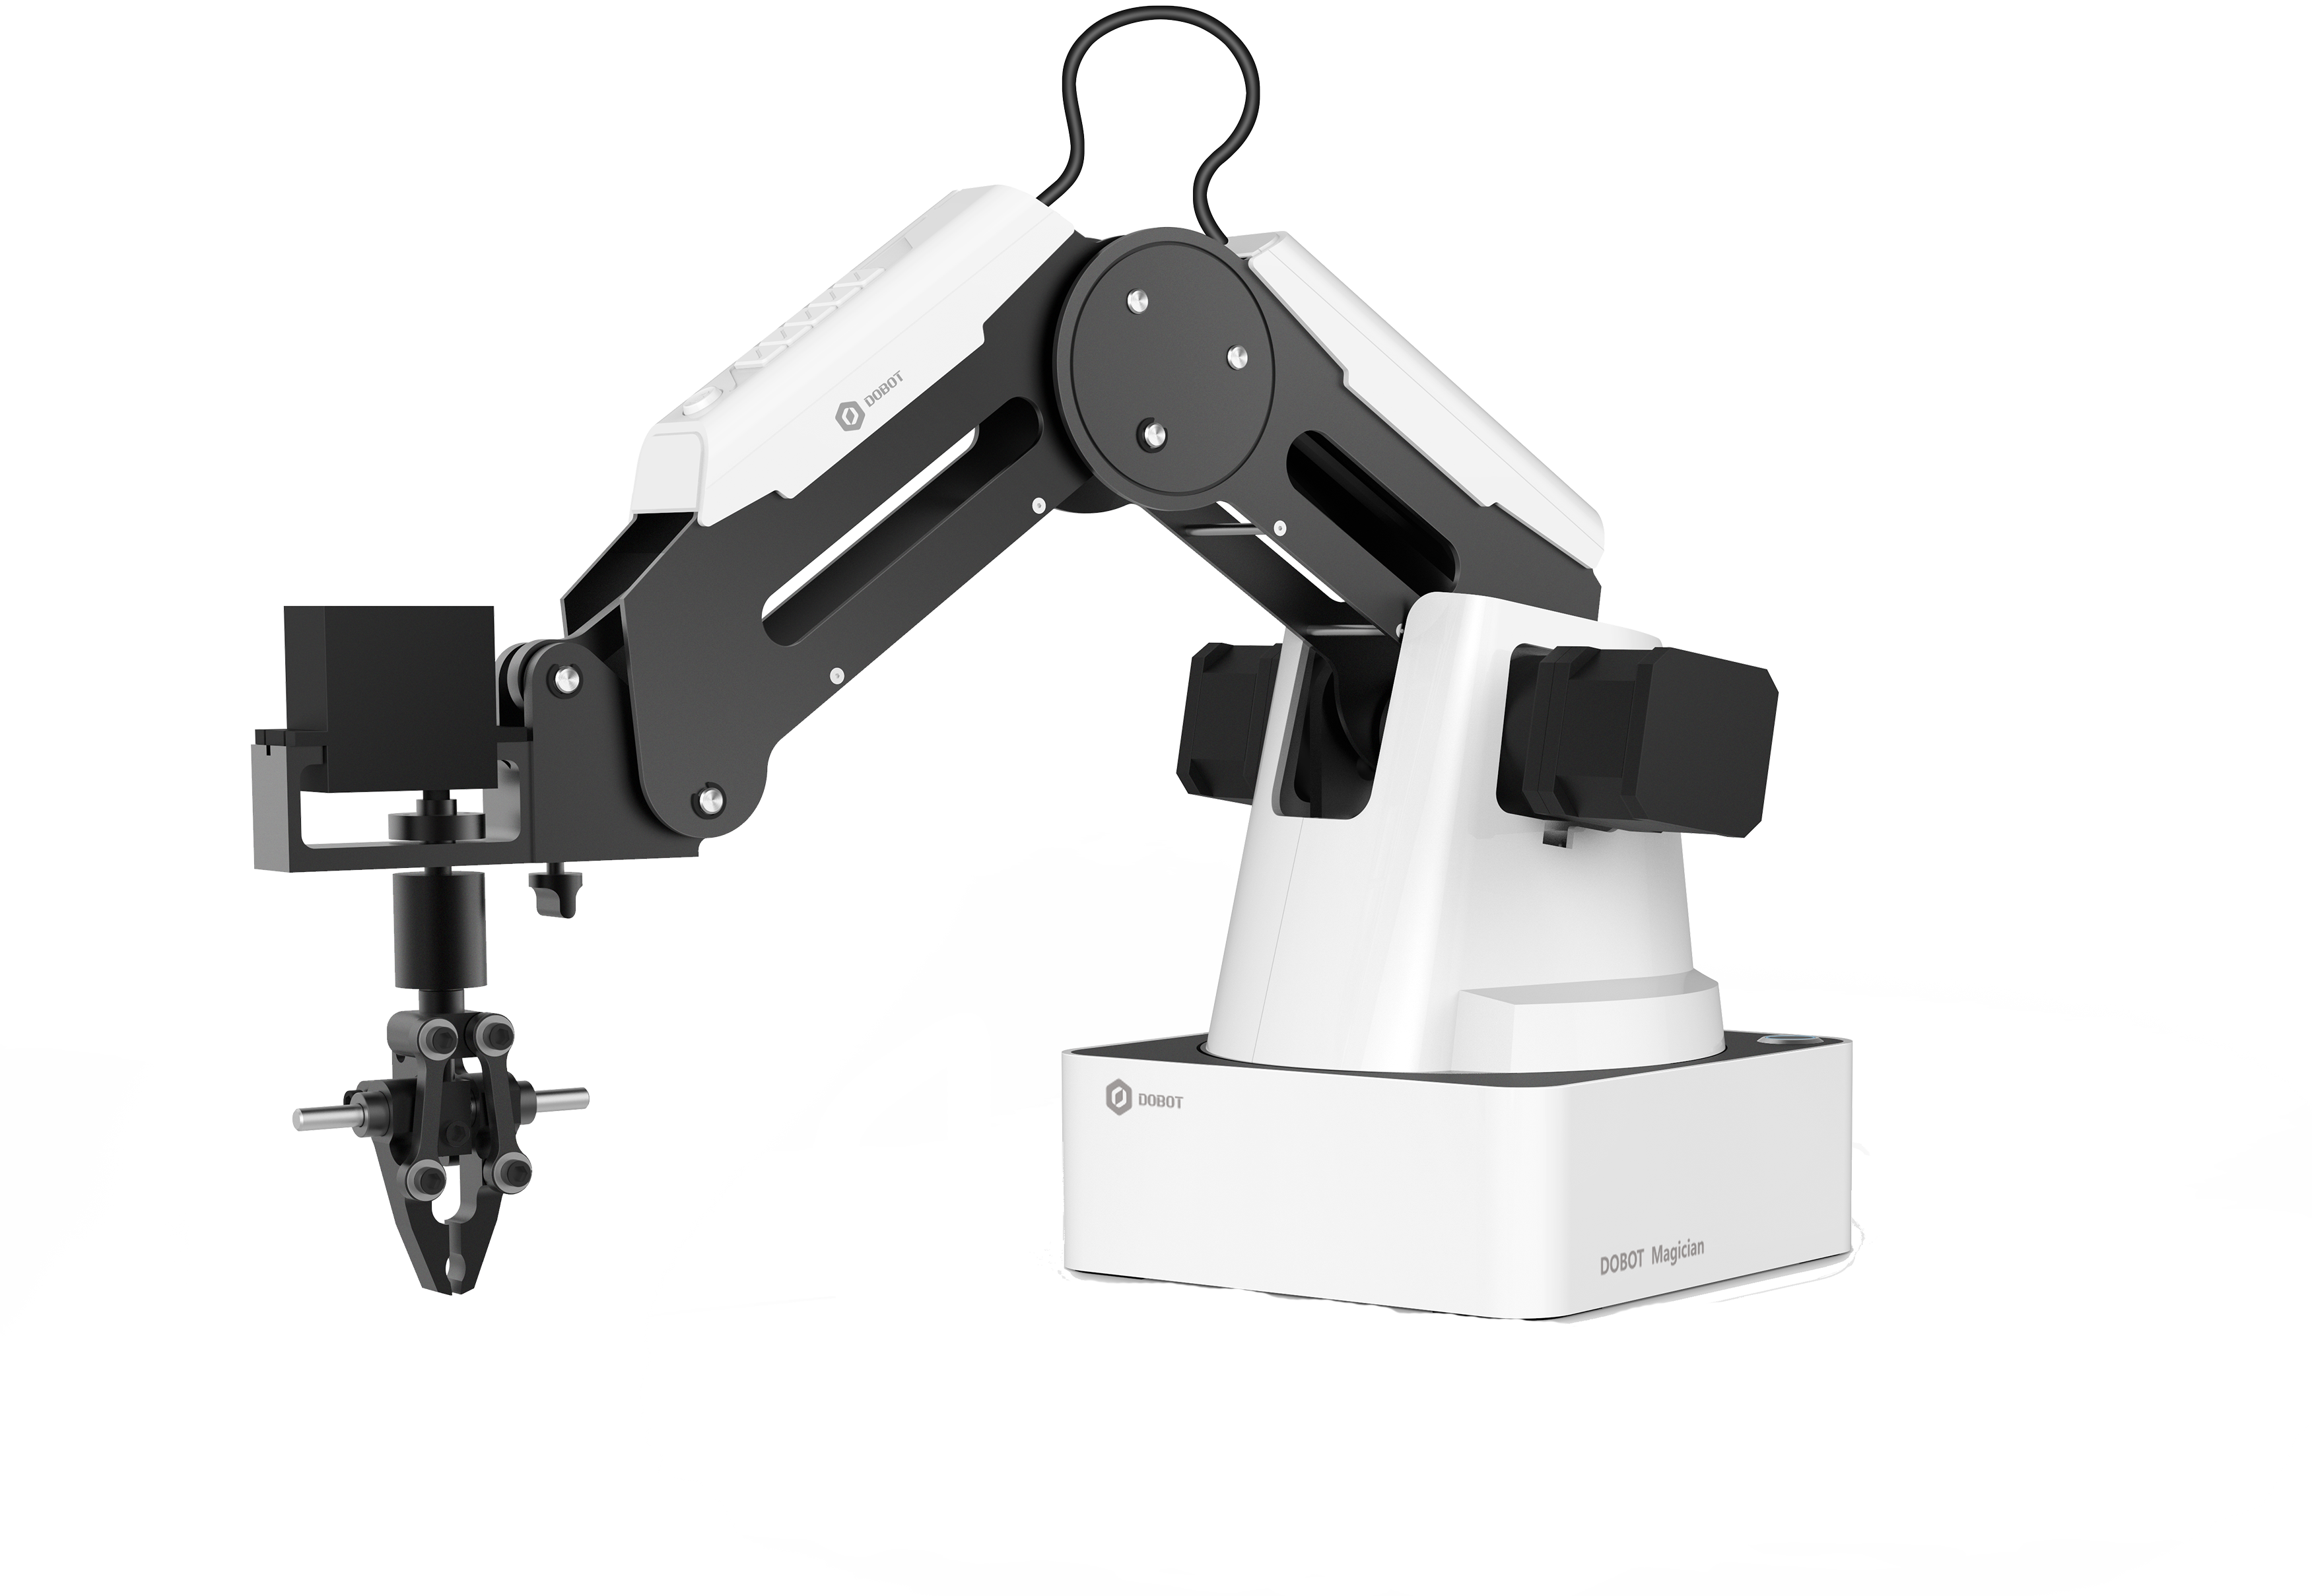
\includegraphics[width=0.5\linewidth]{figs/dobot.png}}
  \caption{Robots usados en universidades}
\end{figure}


\section{Robótica de bajo coste}
\label{sec:rob_bajo:coste}
\begin{figure} [ht!]
  \centering    
  \subfigure[OSTR \footnote{\url{https://www.instructables.com/Low-Cost-Arduino-Compatible-Drawing-Robot/}}]{\label{fig:osrt}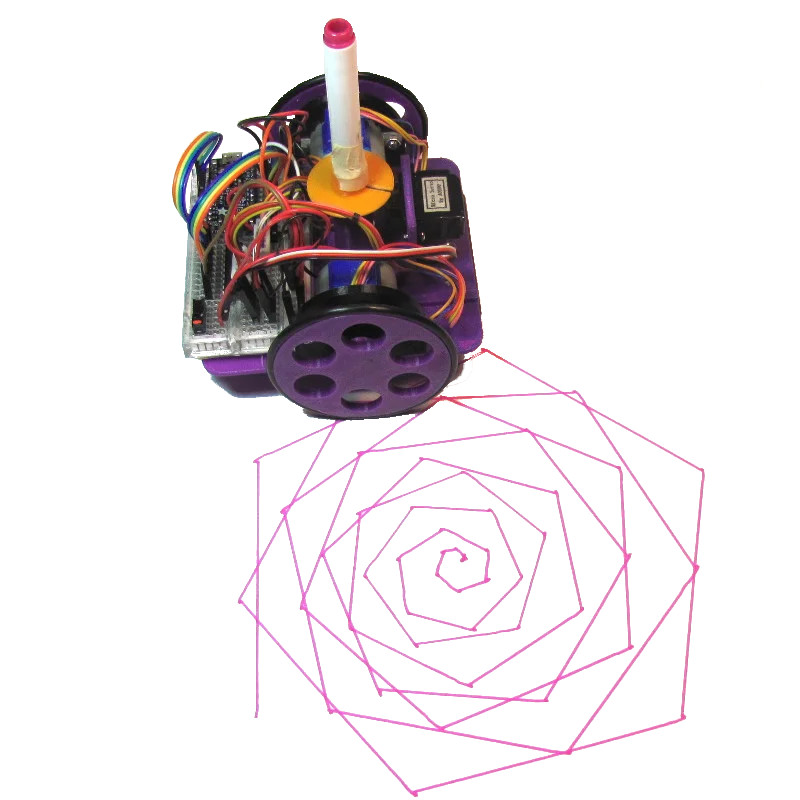
\includegraphics[width=0.4\linewidth ]{figs/OSTR.jpg}}
  \hspace{1cm}
  \subfigure[Dobot Magician \footnote{\url{https://www.robotlab.com/store/dobot-robotic-arm}}]{\label{fig:dobot}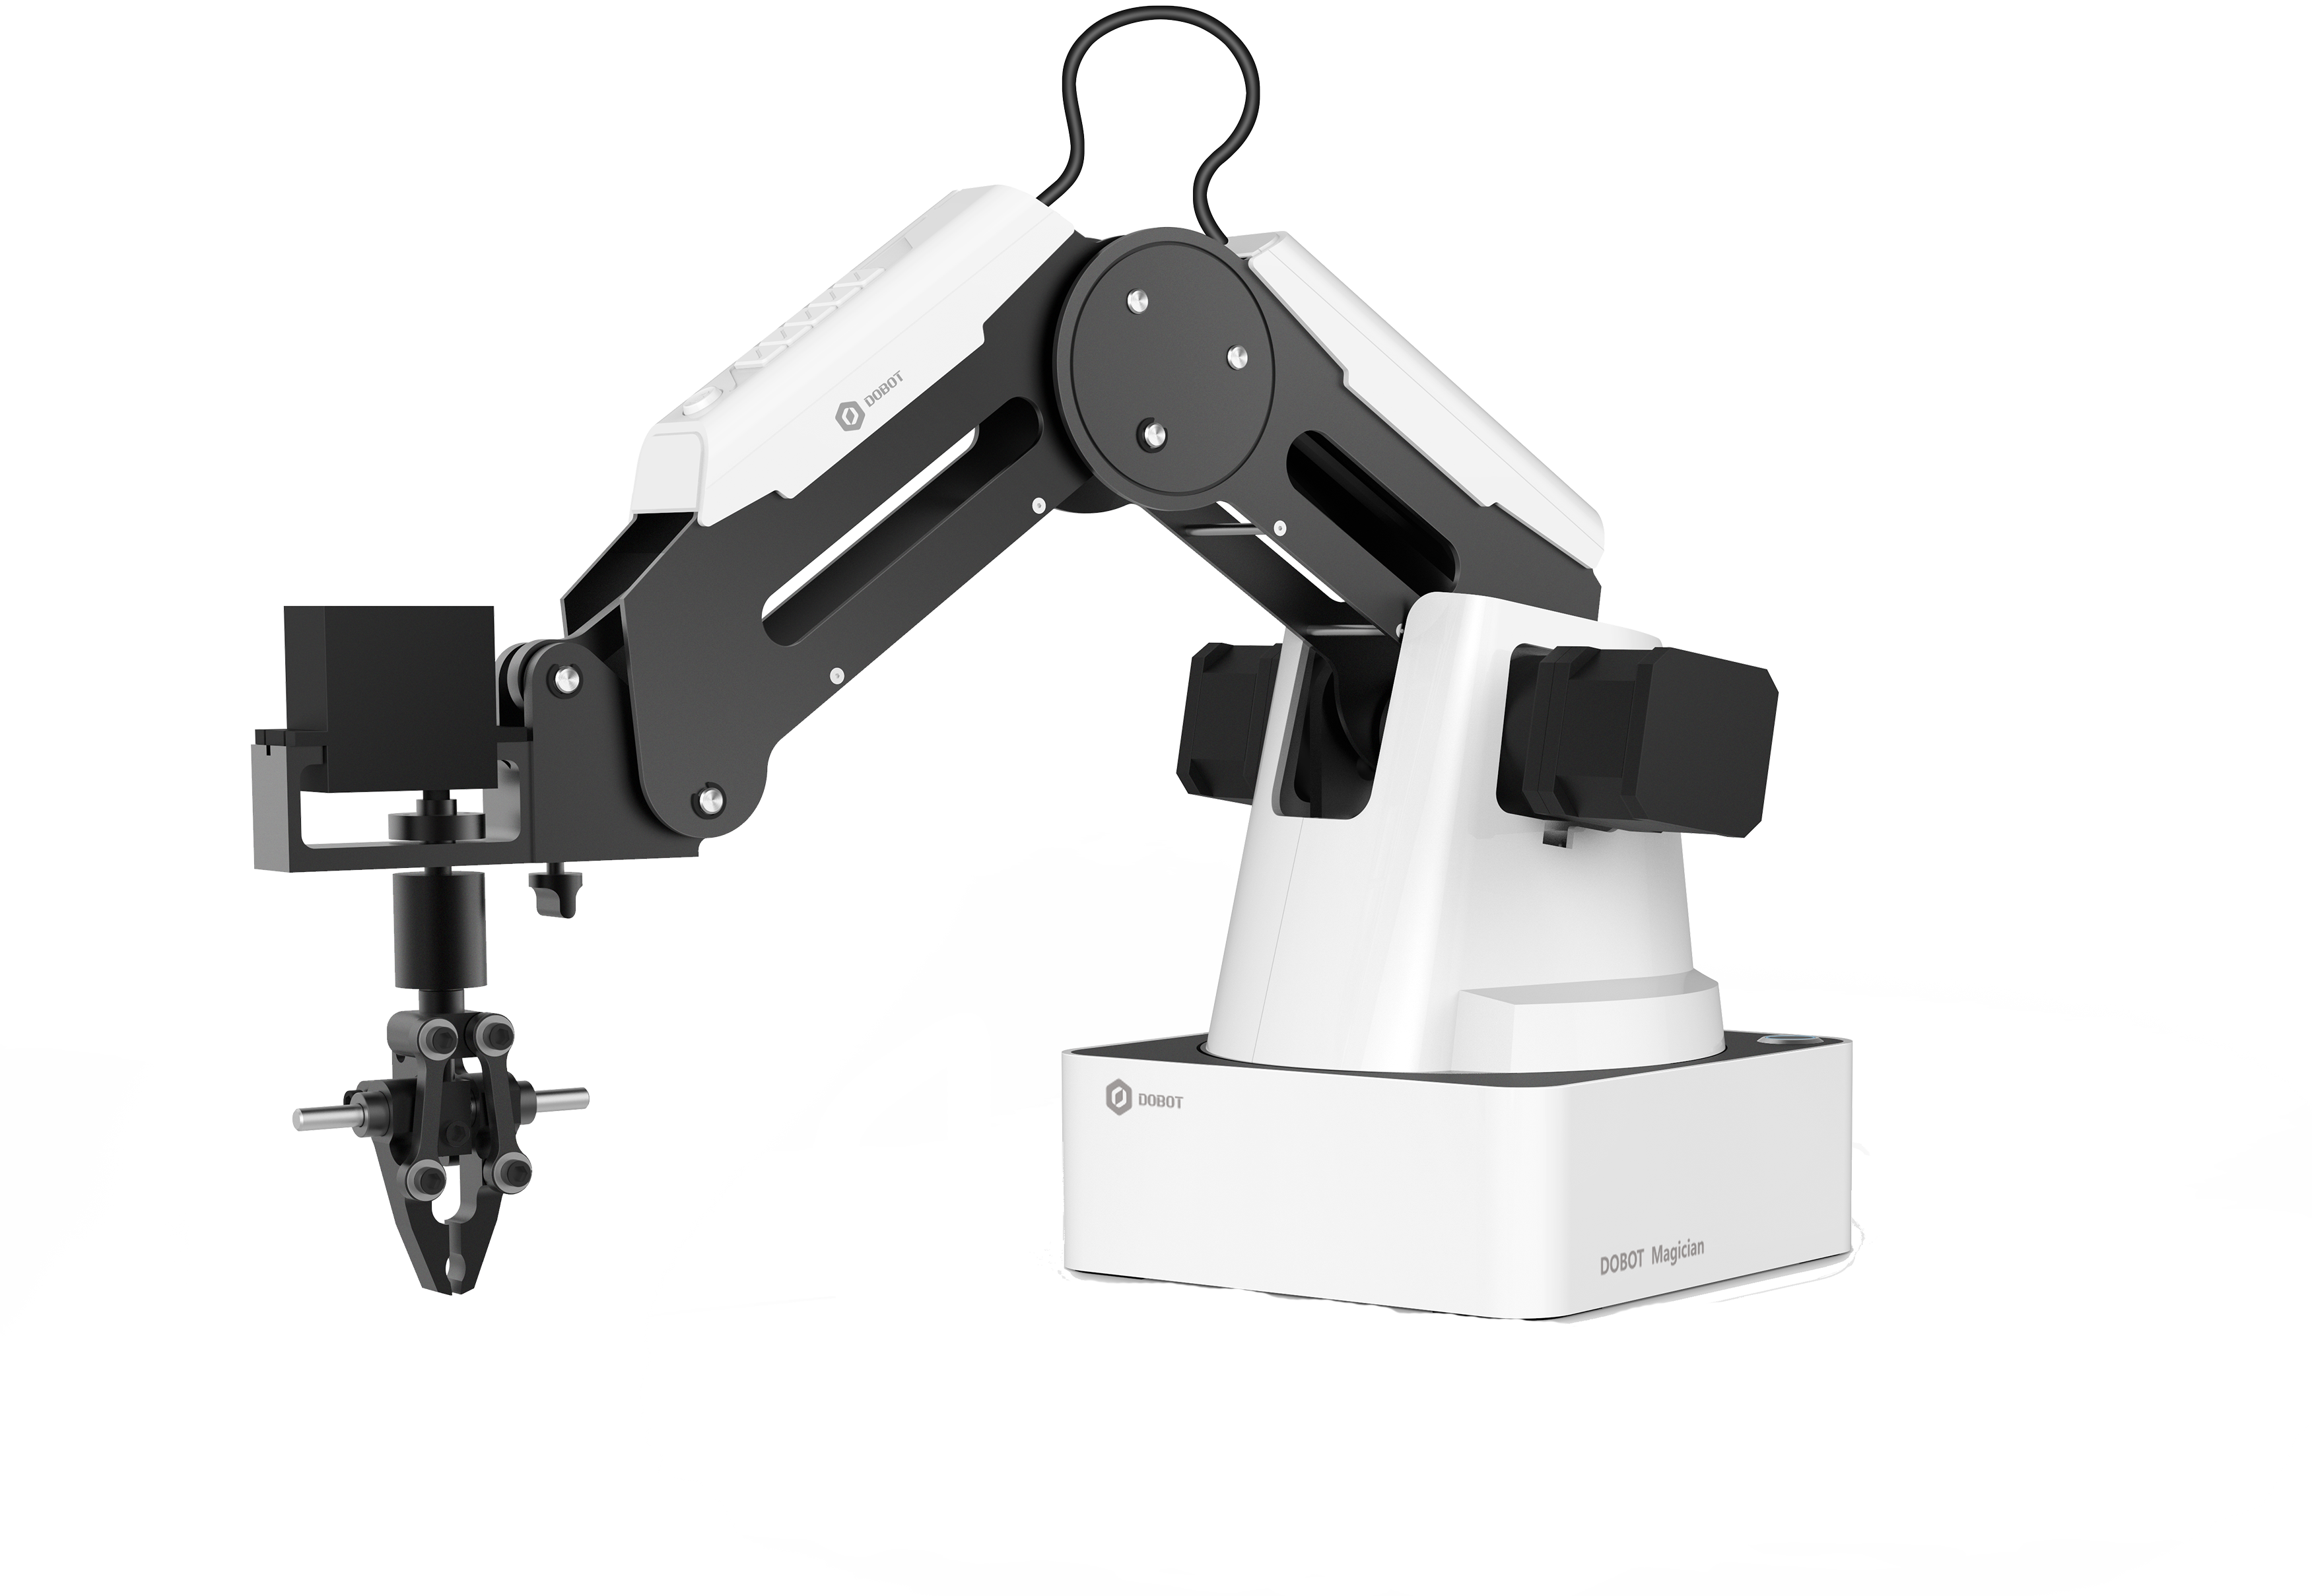
\includegraphics[width=0.5\linewidth]{figs/dobot.png}}
  \caption{Robots usados en universidades}
\end{figure}






Estado del arte
https://www.active-robots.com/our-blog/niryo-ned-robot/
